\documentclass[output=paper]{langscibook}
\ChapterDOI{10.5281/zenodo.4729802}

\author{Céline Pozniak\affiliation{Université Paris 8, Structures Formelles du Langage, CNRS} and 
        Anne Abeillé\affiliation{Université de Paris, Laboratoire de linguistique formelle} and  
        Barbara Hemforth\affiliation{Université de Paris, Laboratoire de linguistique formelle, CNRS}}
\title{Subject inversion in French object relatives: What’s your preference?}


\abstract{\begin{sloppypar} Subject inversion in French is usually
    considered to be optional \citep{LeBidoisR1950,kayne1978} and more
    costly than variants with preverbal subject. As the result of verb
    movement \citep{HulkPollock2001}, it is claimed to demand higher
    processing cost \citep{Holmes1981}.  However, some studies suggest
    that subject inversion in relative clauses may even be favoured by
    certain semantic or heaviness constraints \citep{Fuchs2006,
      marandin2011}. In this paper, we take an empirical approach to
    this question. In our corpus study using the French Treebank
    described in \citet{abeille2019corpus}, we found that subject
    inversion in object relatives can be as frequent as cases without
    inversion. We also found that inversion is preferred with longer
    subjects and shorter and non-agentive verbs. This pattern was
    confirmed in an acceptability judgement experiment as well as in a
    self-paced reading experiment. Thus, object relatives with and
    without inversion are not merely stylistic variants (i.e. two
    equivalent syntactic ways of expressing one meaning), but are more
    or less preferred depending on their properties. Our results are
    compatible with semantic accounts of relative clause processing
    \citep{mak2006animacy, traxler2002}.\end{sloppypar}}


\begin{document}
\maketitle


\section{Introduction} 
French object relative clauses (ORs) are introduced by \textit{que} and may have a preverbal (\ref{ex:OR-inv}) or a postverbal subject (\ref{ex:OR+inv})  \citep{LeBidoisR1950, kayne1978}.


\begin{exe}
\ex Object relative with preverbal subject\label{ex:OR-inv}\\ 
\gll Le médecin [que l'avocat{\tiny subj} connaît] aime courir.\\   
the physician that {the lawyer} knows likes run\\
\glt `The physician [that the lawyer knows] likes running.'

\ex Object relative with postverbal subject\label{ex:OR+inv}\\  
\gll Le médecin [que connaît l'avocat{\tiny subj}] aime courir.\\    
the physician that knows {the lawyer}  likes run\\
\glt `The physician [that the lawyer knows] likes running.'
\end{exe}


In this paper, we will address the question of the status of these two
types of object relatives. Are they just stylistic variants or do they
differ with respect to specific properties beyond subject-verb order?
We will conclude from our empirical studies that specific properties
make each of them more or less felicitous, thus contributing to the
many (variants) to one (meaning) aspect of this volume. We will also
show that the choice of a (one) particular object relative structure
depends on the combination of (possibly many) factors.

\begin{sloppypar}
  Object relatives with a preverbal subject (OR$-$inv) are considered
  canonical while object relatives with a postverbal subject
  (OR$+$inv) are often seen as marked and as a stylistic variant
  (especially for written French).  According to semantic and
  pragmatic theories, the postverbal subject is generally thought of
  as having properties different from a preverbal subject: the
  postverbal subject is more likely to be indefinite and focal
  \citep{Lahousse2011} and/or long and not agentive \citep{Fuchs2006,
    marandin2011}.  Syntactic theories usually consider subject
  inversion as more complex, and the result of verb movement
  \citep{deprez1990two, HulkPollock2001} or specific linearization
  rules \citep{Bonami}. However, an inversion analysis may be favored in
  relativized minimality \citep{rizzi1990, Friedmann2009}, where a
  preverbal animate subject may interfere with the filler-gap
  dependency (\ref{ex:OR-inv2}), which can be avoided with a
  postverbal subject (\ref{ex:OR+inv2}).
\end{sloppypar}

\begin{exe}
\ex OR$-$inv \label{ex:OR-inv2}\\ 
\gll le médecin [que l'avocat connaît \_\_ ] \\   
the physician that {the lawyer} knows \_\_ \\
\glt `the physician [that the lawyer knows \_\_ ]'

\ex OR$+$inv \label{ex:OR+inv2}\\ 
\gll le médecin [que connaît \_\_ l'avocat]\\    
the physician that knows \_\_ {the lawyer} \\
\glt `the physician [that knows \_\_ the lawyer]'
\end{exe}

As for processing theories, differences in linear distance predict
that OR$+$inv should be easier to process than OR$-$inv. According to
dependency locality theory \citep{gibson2000}, the linear distance
between the filler (\textit{que}) and the object gap is shorter in
OR$+$inv (\ref{ex:OR+inv2}), leading to a lower storage memory cost than
in OR$-$inv (\ref{ex:OR-inv2}). The distance is also shorter between the
filler (\textit{que}) and the relative clause verb (\textit{connaît})
if we consider traceless theories of extraction, with a \textsc{slash} feature
on the verb \citep{BoumaSag2001, sag2010}.

Two (complementary) approaches will be applied in order to put these
theories and their conflicting predictions to an empirical test. The
first is to look at large corpora, to see how frequent subject
inversion is in object relative clauses, and which factors may favour
or disfavour it. The second way is to conduct experiments that enable us
to test these factors in a controlled environment. In this paper, we
will associate corpus studies and experiments in order to provide
converging evidence.  Previous corpus studies on newspaper texts found
a 41\% inversion rate for French relative clauses
\citep{catherine1997}. \citet{catherine1997} conducted a corpus study
on one issue of the newspaper \textit{Le Monde} and found that
relatives with a nominal subject (not only object relative clauses but
including those with \textit{dont} `whose', \textit{où} `where') were
more frequent with a preverbal subject than with a postverbal
subject. Based on the frequency distribution in her corpus, she
suggests that subject inversion is favoured when the subject is not
agentive, inanimate and definite, when it is longer than the verb
phrase and when the verb is not agentive. While our own corpus studies
will be strongly inspired by Fuchs’s analysis, we will
restrict our analysis to object relative clauses but also go beyond
their approach by testing the different constraints as well as their
intercorrelations using state of the art inferential statistics.

On the processing side, previous experimental studies found that
object relatives with postverbal subject were more difficult to
understand than those with preverbal subject. In an eye-tracking experiment,  \citet{Holmes1981}
examined participants' eye movements while they read sentences with animate
subjects and objects and reversible verbs (\textit{dessiner} ‘draw’,
\textit{voir} ‘see’, …).  \citet{pozniak2015processing}, also using
animate subjects and reversible verbs, conducted an eye-tracking
experiment using the visual world paradigm, where participants listened to 
sentences including subject relative clauses as well as
object relative clauses with postverbal (\ref{OR+inv3}) or with
preverbal subject (\ref{OR-inv3}) while they saw two pictures on a
computer screen, one compatible with a subject relative clause
interpretation (where the princess draws the fencer) and the other one
compatible with an object relative clause interpretation (where the
fencer draws the princess). The participants’ task was to look at the
``correct'' picture, i.e. the picture compatible with the sentence they
heard, on a computer screen. More and earlier fixations on the correct
picture are interpreted as evidence for easier processing in this
paradigm.


\begin{exe}
\ex OR$-$inv \label{OR-inv3}\\ 
\gll {Prière de} trouver la princesse correcte, c'est-à-dire la belle princesse [que l'escrimeur dessine] sur l'image. \\ please find the princess correct, {that is to say} the beautiful princess that {the fencer} draws on {the picture}\\ 
\glt `Please find the correct princess, that is to say the beautiful princess [that the fencer draws] on the picture.'

\ex OR$+$inv \label{OR+inv3}\\ 
\gll {Prière de} trouver la princesse correcte, c'est-à-dire la belle princesse [que dessine l'escrimeur] sur l'image. \\   please find the princess correct, {that is to say} the beautiful princess that  draws {the fencer} on {the picture}\\ 
\glt `Please find the correct princess, that is to say the beautiful princess [that the fencer draws] on the picture.'
\end{exe}


Subject relative clauses, which were tested in both the
\citet{Holmes1981} reading experiment and the visual world
eye-tracking experiment by \citet{pozniak2015processing}, were
processed faster and led to more fixations on the correct image than
both object relative clause variants. However, both studies also found
that OR$+$inv were more difficult to process than OR$-$inv, contrary to
what is predicted by processing theories like DLT or syntactic
theories like relativized minimality.  Processing data from
experiments also provide evidence for more fine-grained semantic
constraints: \citet{Frauenfelder1980} compared OR$+$inv with reversible
verbs (\textit{connaître} `know’) and animate objects
(\ref{animateobject}) vs. with non-reversible verbs
(\textit{publier} `publish’) and inanimate objects
(\ref{inanimateobject}). Using a phoneme monitoring task (where
participants have to press a button as soon as they hear a particular
phoneme), they found that OR$+$inv was easier with inanimate objects
(\ref{inanimateobject}) than with animate objects. However, their data
cannot tell us whether these factors are specific to object relatives
with a postverbal subject (OR$+$inv) or concern object relatives in
general, since this study did not include a comparison of ORs with
postverbal and preverbal subject.

\begin{exe}
\ex \label{animateobject}
\gll Le savant [que connaît le docteur] travaille dans une université moderne.\\   
 the scientist that knows the doctor works in a university modern \\
\glt `The scientist [that the doctor knows] works in a modern university.'

\ex \label{inanimateobject}
\gll Les articles [que publie la revue] demandent une lecture attentive.\\    
 the articles that publishes the journal {ask for} a reading careful\\
\glt `The articles [that the journal publishes] demand a careful reading.'
\end{exe}


Using eye-tracking while reading and self-paced reading paradigms,
\citet{baudiffier2011effect} directly compared OR$-$inv and OR$+$inv. They found that 
OR$-$inv were generally easier to process than OR$+$inv with inanimate subjects 
and animate objects.  These experiments mainly
focused on the role of animacy for the two types of relatives, but did
not test length or other semantic or pragmatic properties that have
been suggested to play a role as well \citep [e.g.][]{catherine1997}.

In the following sections, we present a new corpus study, based on a
syntactically annotated corpus \citep [the French
Treebank,][]{abeille2019corpus}, and two new experiments. We found
that OR$+$inv can be as frequent as OR$-$inv, furthermore, they can be
as acceptable as OR$-$inv in two controlled experiments manipulating
semantic/pragmatic properties.


\section{Inversion in object relatives: a corpus study} 


We searched for object relatives in the French Treebank \citep{abeille2019corpus}\footnote{Available on \url{http://ftb.linguist.univ-paris-diderot.fr/}.}, which comprises around 21550 sentences from newspaper texts (\textit{Le Monde} from 1990 to 1993). We extracted object relatives (with \textit{que}) with a nominal subject and obtained 298 ORs in total, 149 of which had a postverbal subject. In order to have a fully parallel comparison for subject inversion, we excluded cleft constructions, appositive relatives, obligatory relatives after demonstratives (\textit{ce que}), relatives with a pronominal subject (\textit{cela} ‘this’, \textit{certains} ‘some’) and some errors (clitic subjects). This leaves 178 object relatives, 90 with subject inversion as in (\ref{excorpusinversion}), and 88 without as in (\ref{excorpusnoinversion}). 

\begin{exe}
\ex \label{excorpusinversion}

\gll …, le conseil régional de Picardie a pris position sur les problèmes [que connaît {l’audiovisuel public} dans la région].\\    
…, the regional council  of Picardy has taken {a stance} on the problems that encounters {the audiovisual media} in the region\\
\glt `…, the regional council  of Picardy has taken a stance on the problems [that encounters the audiovisual media in the region].'


\ex \label{excorpusnoinversion}
\gll Le rôle d'intimidation [que l'armée rouge aura après la démilitarisation de l'Allemagne]…\\    
The role {of intimidation} that {the army} red {will have} after the demilitarization of Germany\\
\glt `The role of intimidation [that the Red Army will have after the demilitarization of Germany] …'

\end{exe}

\subsection{Annotation criteria}
We annotated our 178 object relatives mainly using criteria from Fuchs
\citep{catherine1997, Fuchs2006}. As illustrated in Table
\ref{tab:1:annotation}, we annotated both relatives with animacy of
the subject and the object, relative length between the verb and the
object as well as length of the relative clause, definiteness of the
subject and the object, thematic roles, negation and position of the
relative in the sentence.\footnote{\citet{Fuchs2006} did not mention
  the position of the relative and the negation as criteria for
  subject inversion.}\footnote{The corpus with the annotated
  data can be found on \url{https://osf.io/k97pu/}.}

\begin{table}
\begin{tabular}{ll} 
  \lsptoprule
    Criteria & Annotation\\ 
  \midrule
  Relative &  With preverbal subject \\
& With postverbal subject\\
  Animacy  &   Animate subject and object \\
& Inanimate subject and object \\
& Animate subject and inanimate object \\
& Inanimate subject and animate object \\
Thematic roles & Intentional subject, affected theme \\
& No intentional subject, no affected theme \\
& Intentional subject, no affected theme \\
& No intentional subject, affected theme \\
Verb agentivity & Agentive verb (‘to want’, ‘to fight’) \\
& Non-agentive verb (‘to represent’, ‘to have’) \\ 
Verb/subject length  & Verb longer than subject  \\
(syllables) & Verb shorter than subject \\
& Verb as long as subject \\
Relative clause length & Relative with subject and verb only \\
& Relative with more constituents than verb \\
             &  and subject\\
      Definiteness & Definiteness of the object of the relative \\
& Definiteness of the subject of the relative \\
Negation & Presence of negation \\
& Absence of negation \\
Position of the relative & Inside the main clause subject \\
& Inside the main clause object \\
& Inside another constituent \\
  \lspbottomrule
    \end{tabular}
 \caption{Annotation for object relatives in the corpus\label{tab:1:annotation}}
\end{table}


\subsection{Results}
To analyze the corpus data, we ran logistic regression models using
the \texttt{glmer} function in the \texttt{lme4} R package from \citet{Bates2015}. The
dependent variable was subject inversion, coded as 1 for postverbal
subject (subject inversion) and 0 for preverbal subject (no subject
inversion). The criteria animacy, thematic roles, verb agentivity, verb/subject length,
relative clause length, definiteness, negation, and position of the
relative clause were included as predictors. They were all coded using mean centering.

\begin{sloppypar}
  We used logistic regressions with simple intercepts
  \citep{Jaeger2008} to test whether there is a general difference in
  frequency between the two types of ORs.  No significant difference
  between ORs with preverbal subject and ORs with postverbal subject
  could be established ($z=-0.15, p>0.1$).
\end{sloppypar}

As for the factors we annotated in our corpus (subject definiteness,
negation, animacy, verb agentivity, subject/verb length, relative
clause length, position of the relative and object definiteness), we
decided to run a logistic regression model combining them all as
predictors. It makes sense to analyze them in one model because this
allows us to establish the independent contribution of highly
intercorrelated factors (the factor verb agentivity is linked to
thematic roles, for example). The model including only the
statistically significant predictors is presented in Table
\ref{tab:2:results}. Positive estimates correspond to an increase in
the number of postverbal subjects such that OR$+$inv is more likely for
short ORs with definite objects, non-intentional subjects and with
verbs that are shorter than the subject.

\begin{table}
\caption{Significant factors with logistic regression model for subject inversion. The intercept corresponds to indefinite object/short relative/verb longer than subject/non-intentional subject.}
\label{tab:2:results}
 \begin{tabular}{ l D{.}{.}{2.5} D{.}{.}{2.5}
   D{.}{.}{2.5} D{.}{.}{1.2}}
  \lsptoprule
  Fixed effects	 & \multicolumn{1}{c}{E}  & \multicolumn{1}{c}{SE}    & \multicolumn{1}{c}{$z$}    &	\multicolumn{1}{c}{$p<$}\\ 
  \midrule
  Intercept     & -0.03606 	&     0.19566 	    & -0.184     &  0.1 \\
  Definite object    &  1.25588  &   0.47194         &  2.661     & 0.01 \\
  Long relative       &  1.04969  &  0.41009          &  2.560    &	0.05 \\
Verb shorter than subject   &  1.48045  &   0.63099         &  2.346    &	0.05 \\
Intentional subject         & -1.45056   &   0.55517         & -2.613    &	0.01 \\
  \lspbottomrule
 \end{tabular}
\end{table}


The factors that did not significantly contribute to the model are the
following: position of the relative clause (inside main clause subject
or main clause object), animacy of subject or object, affected theme
and verb agentivity. However, the fact that verb agentivity did not
contribute significantly to the model can be explained by the fact
that an agentive verb needs an intentional subject, so these
predictors are highly correlated ($r=0.6, t=10.08, p<0.001$). The independent
variables that significantly influence subject inversion are
shown in Figure \ref{figcorpus}.

\begin{figure}
\subfigure[Relative Length]{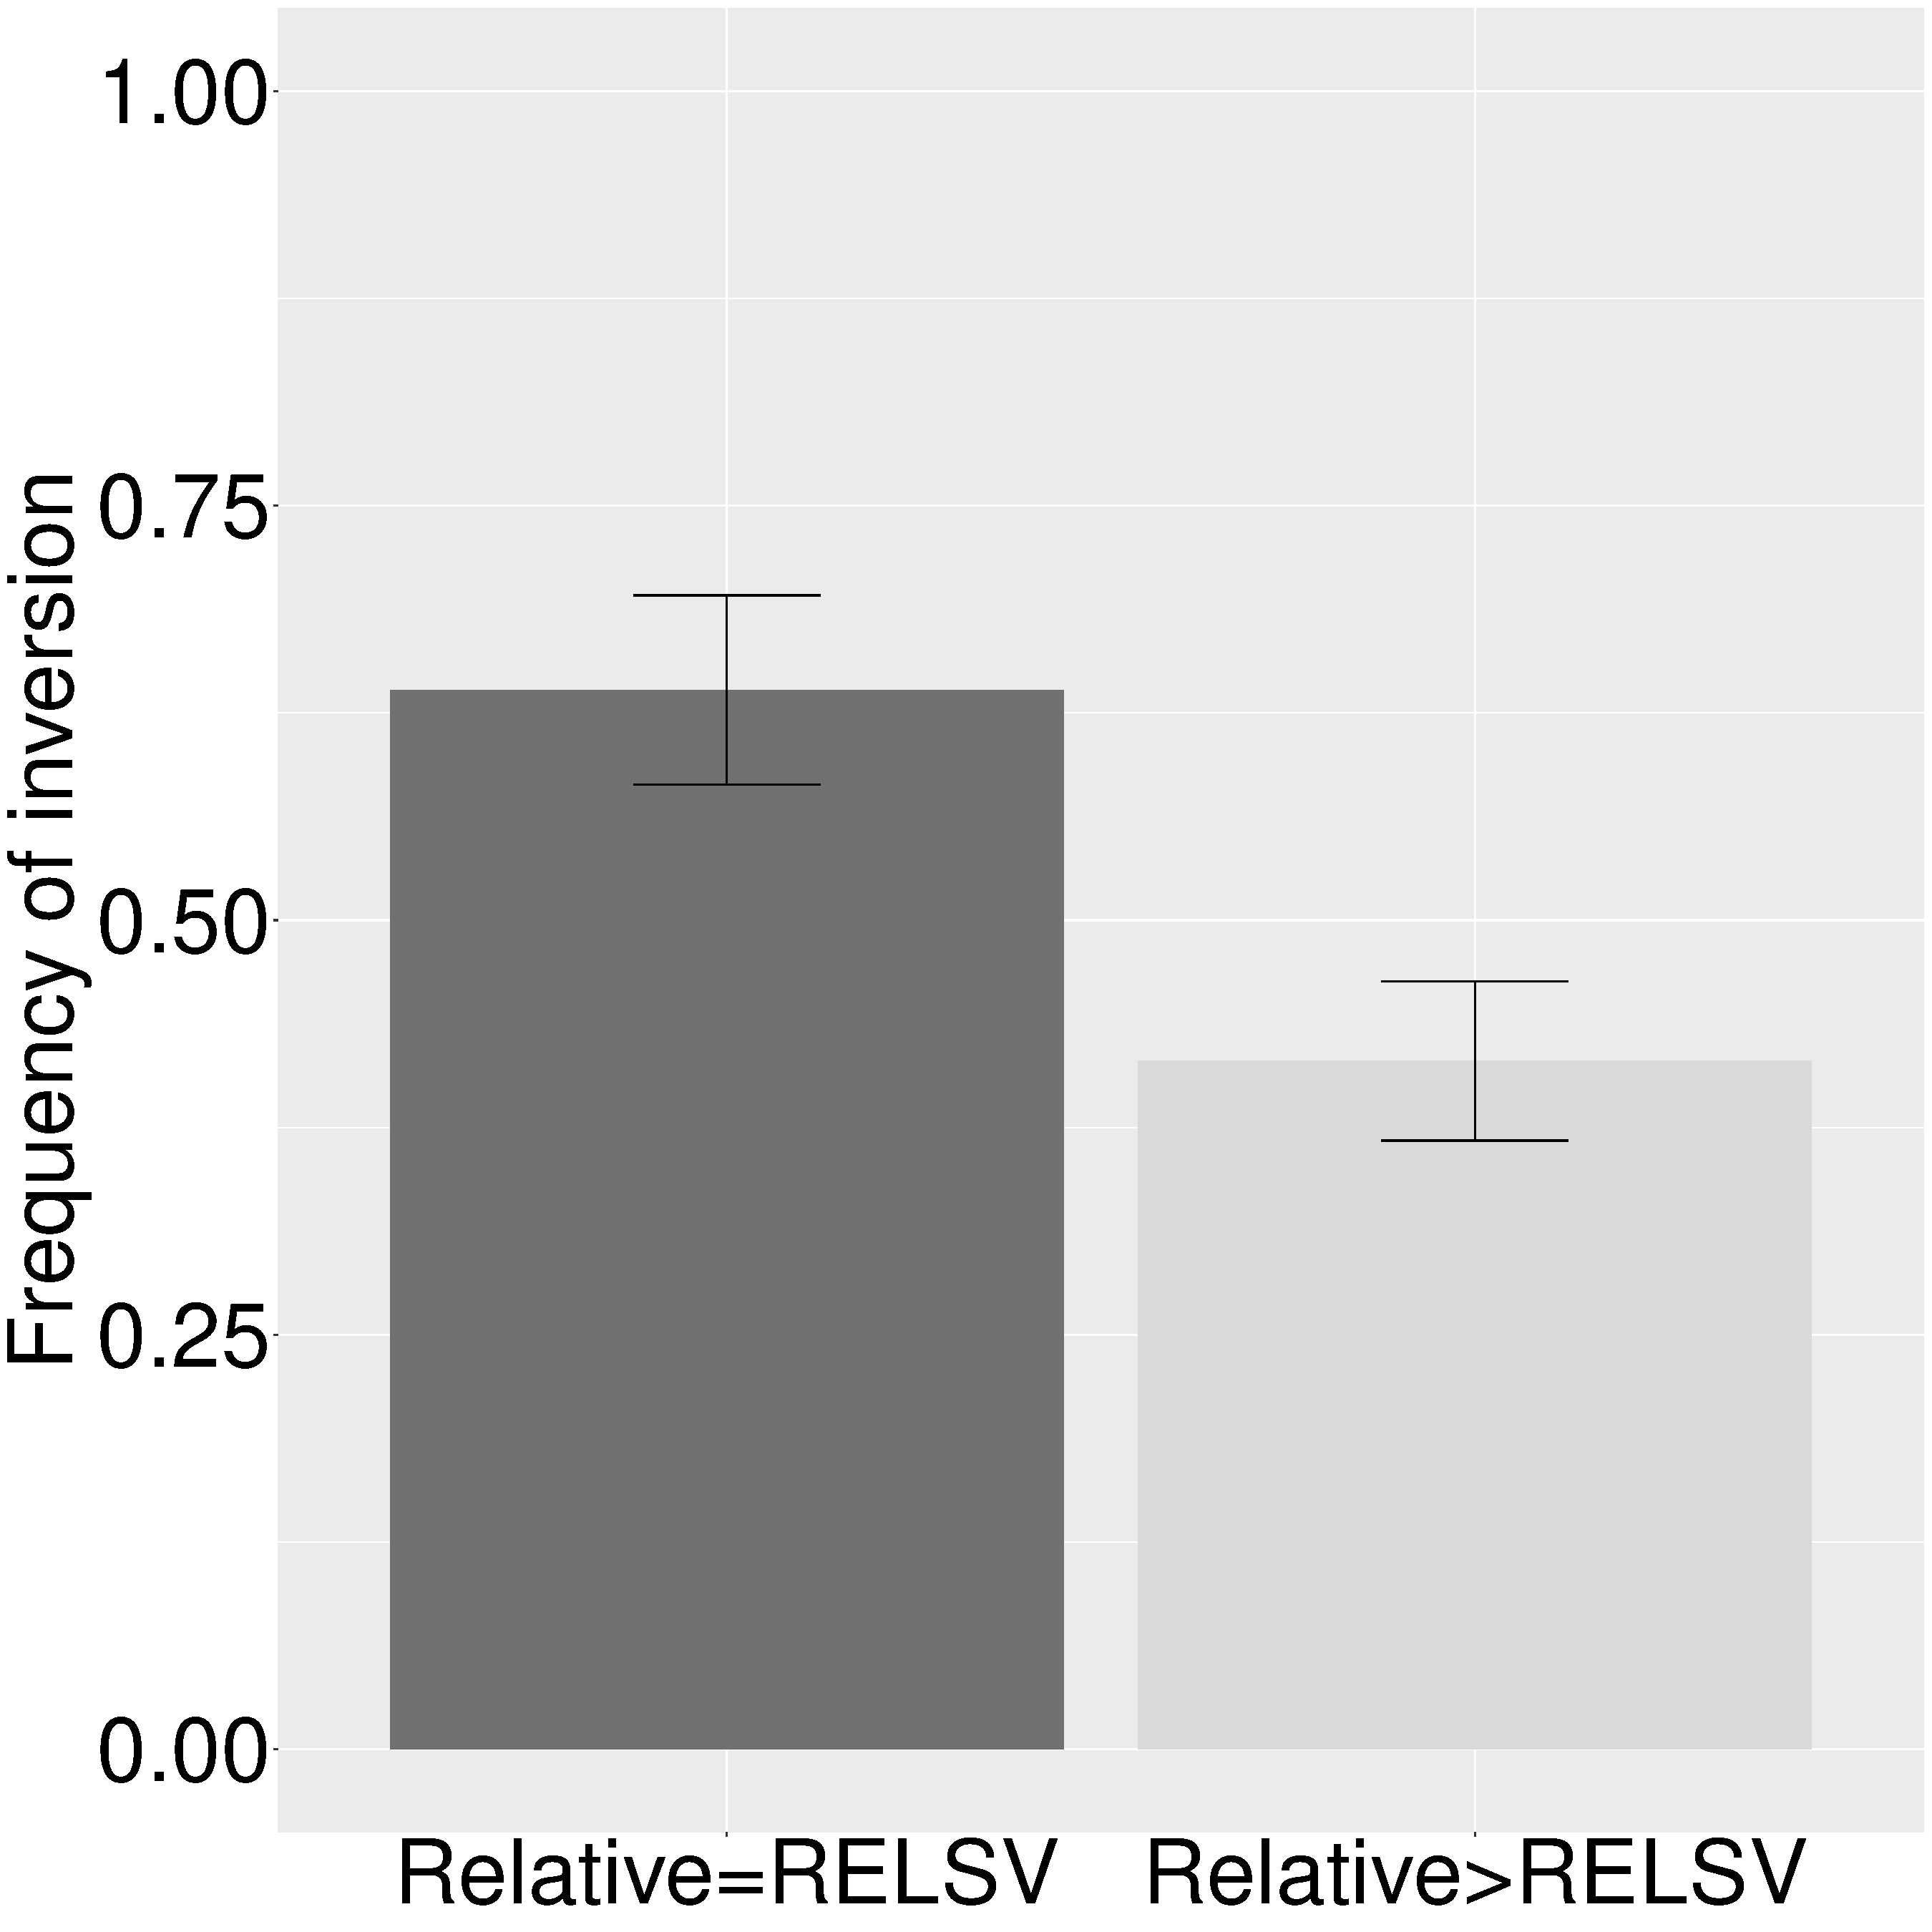
\includegraphics[width = .48\linewidth]{figures/pozhemab1.pdf}} 
\subfigure[Intentional Subject]{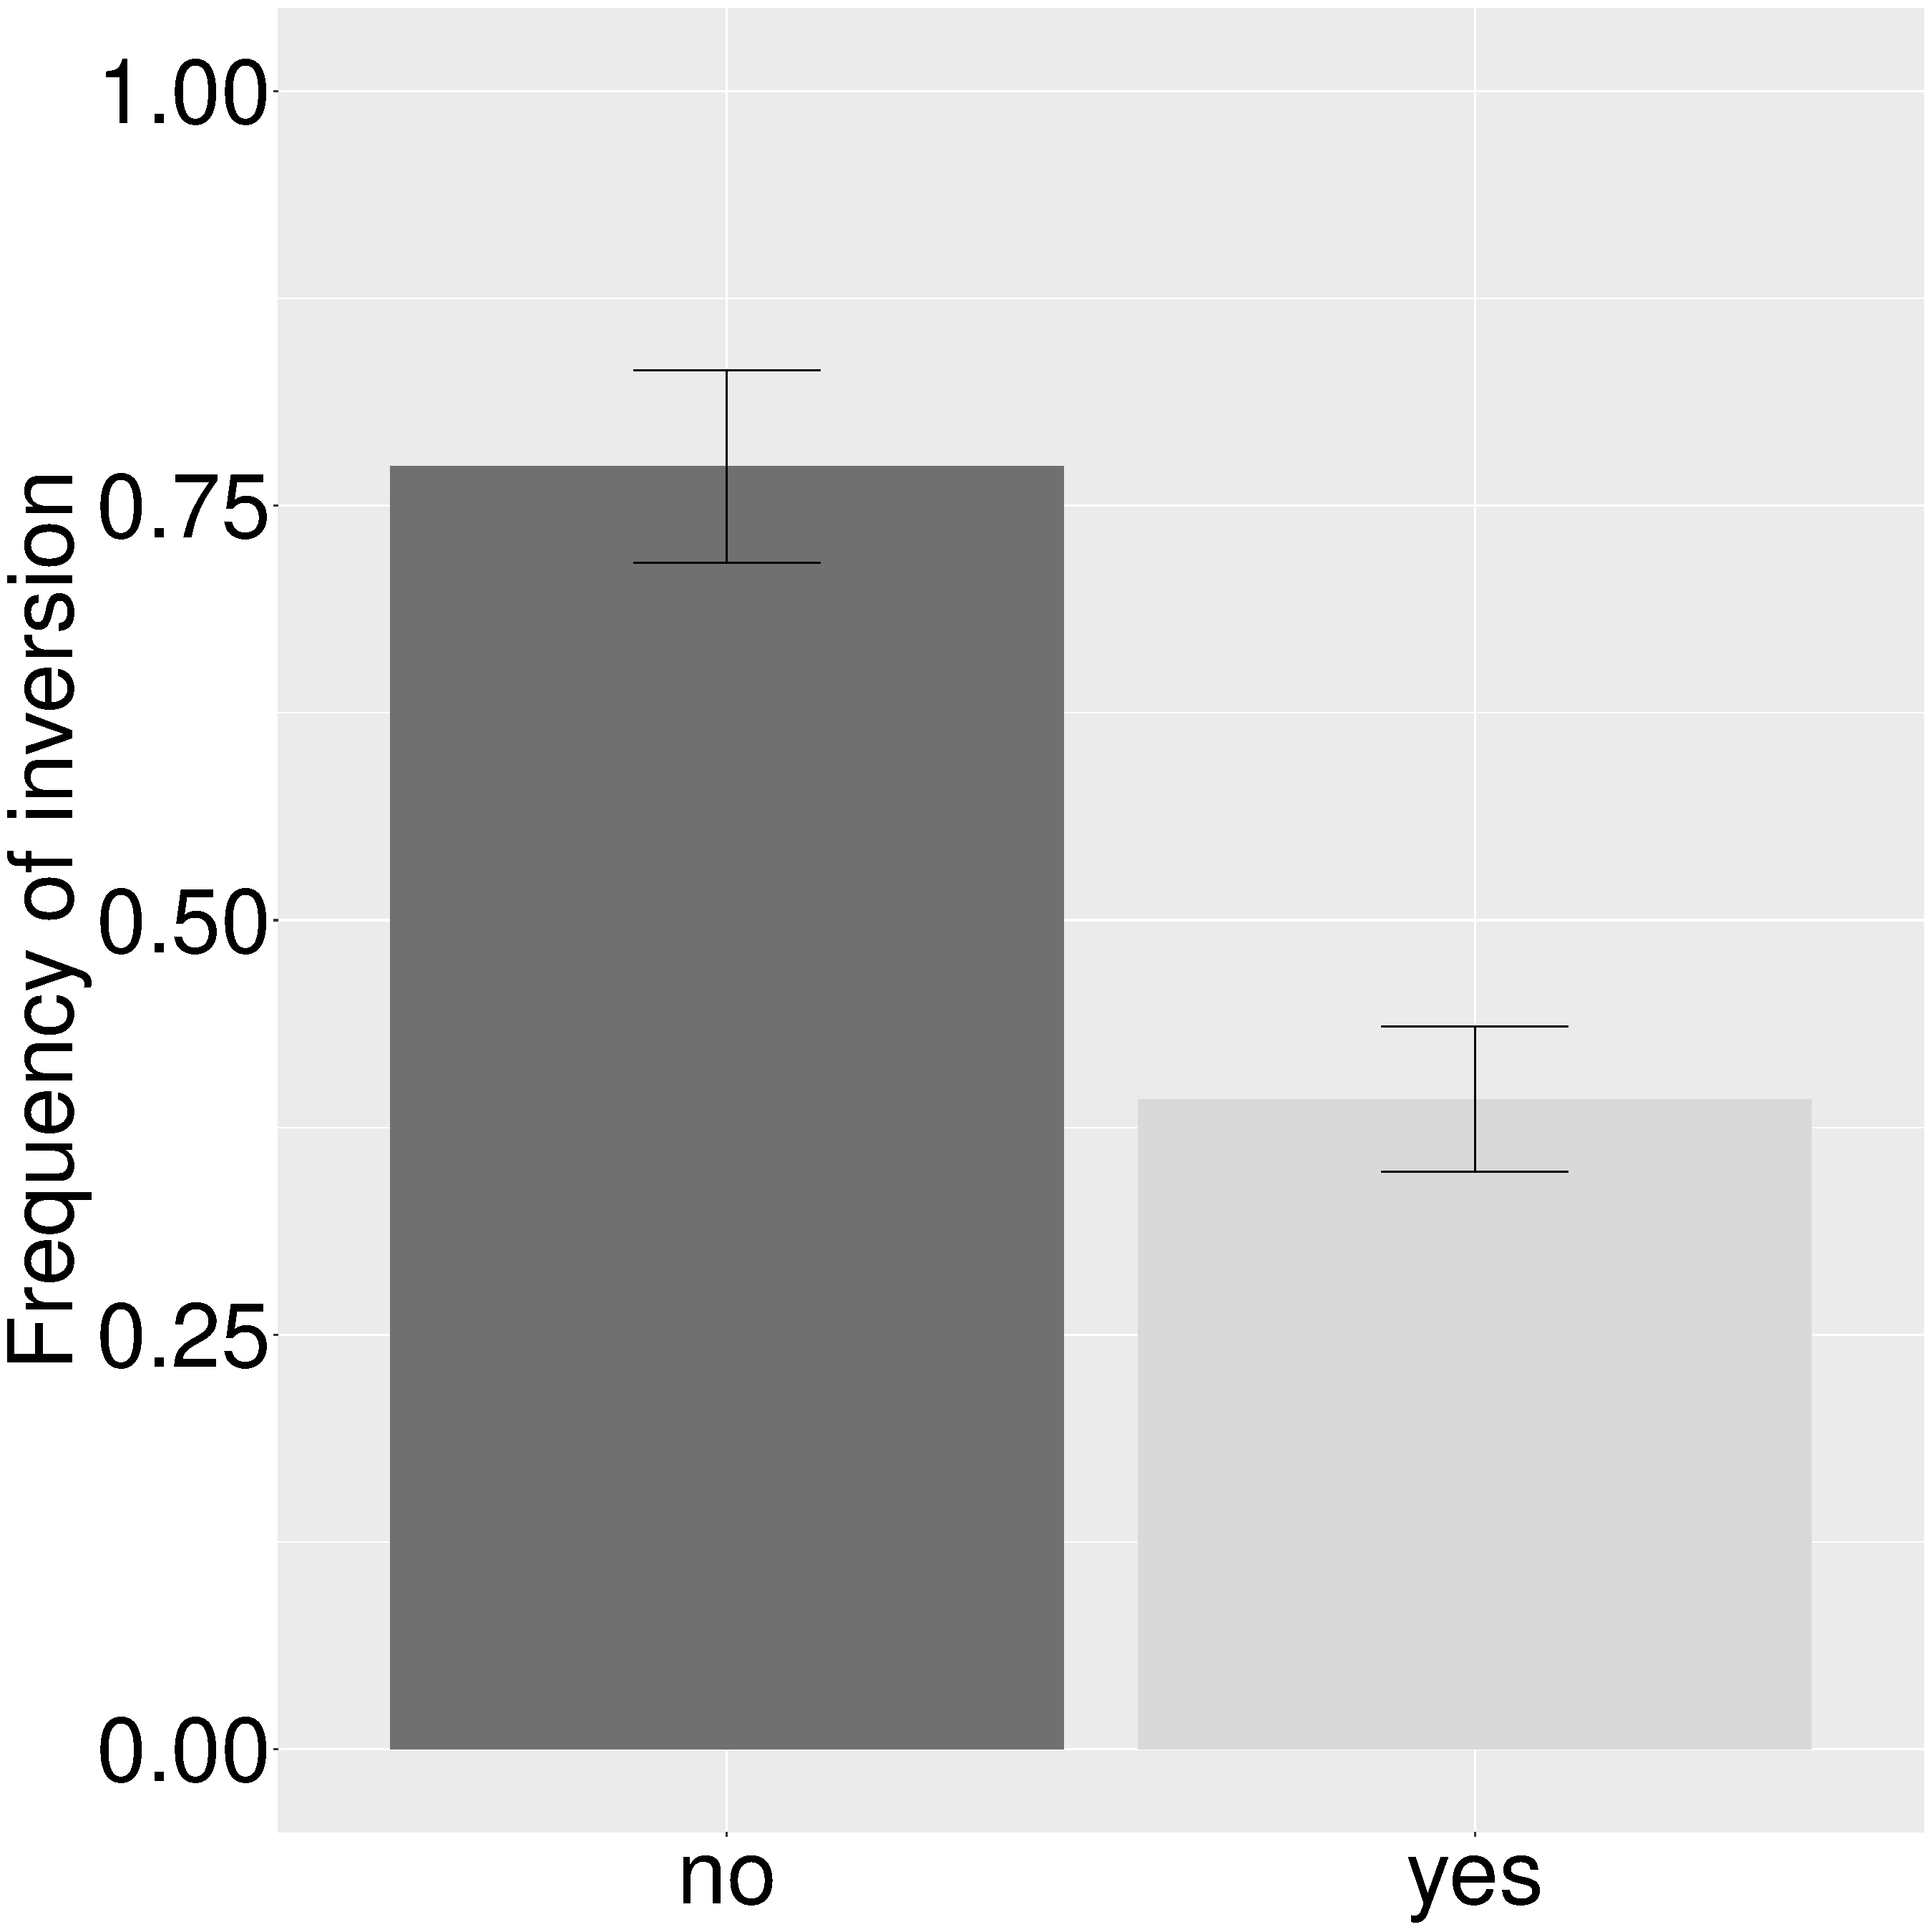
\includegraphics[width = .48\linewidth]{figures/pozhemab2.pdf}}\\
\subfigure[Subject and Verb Length]{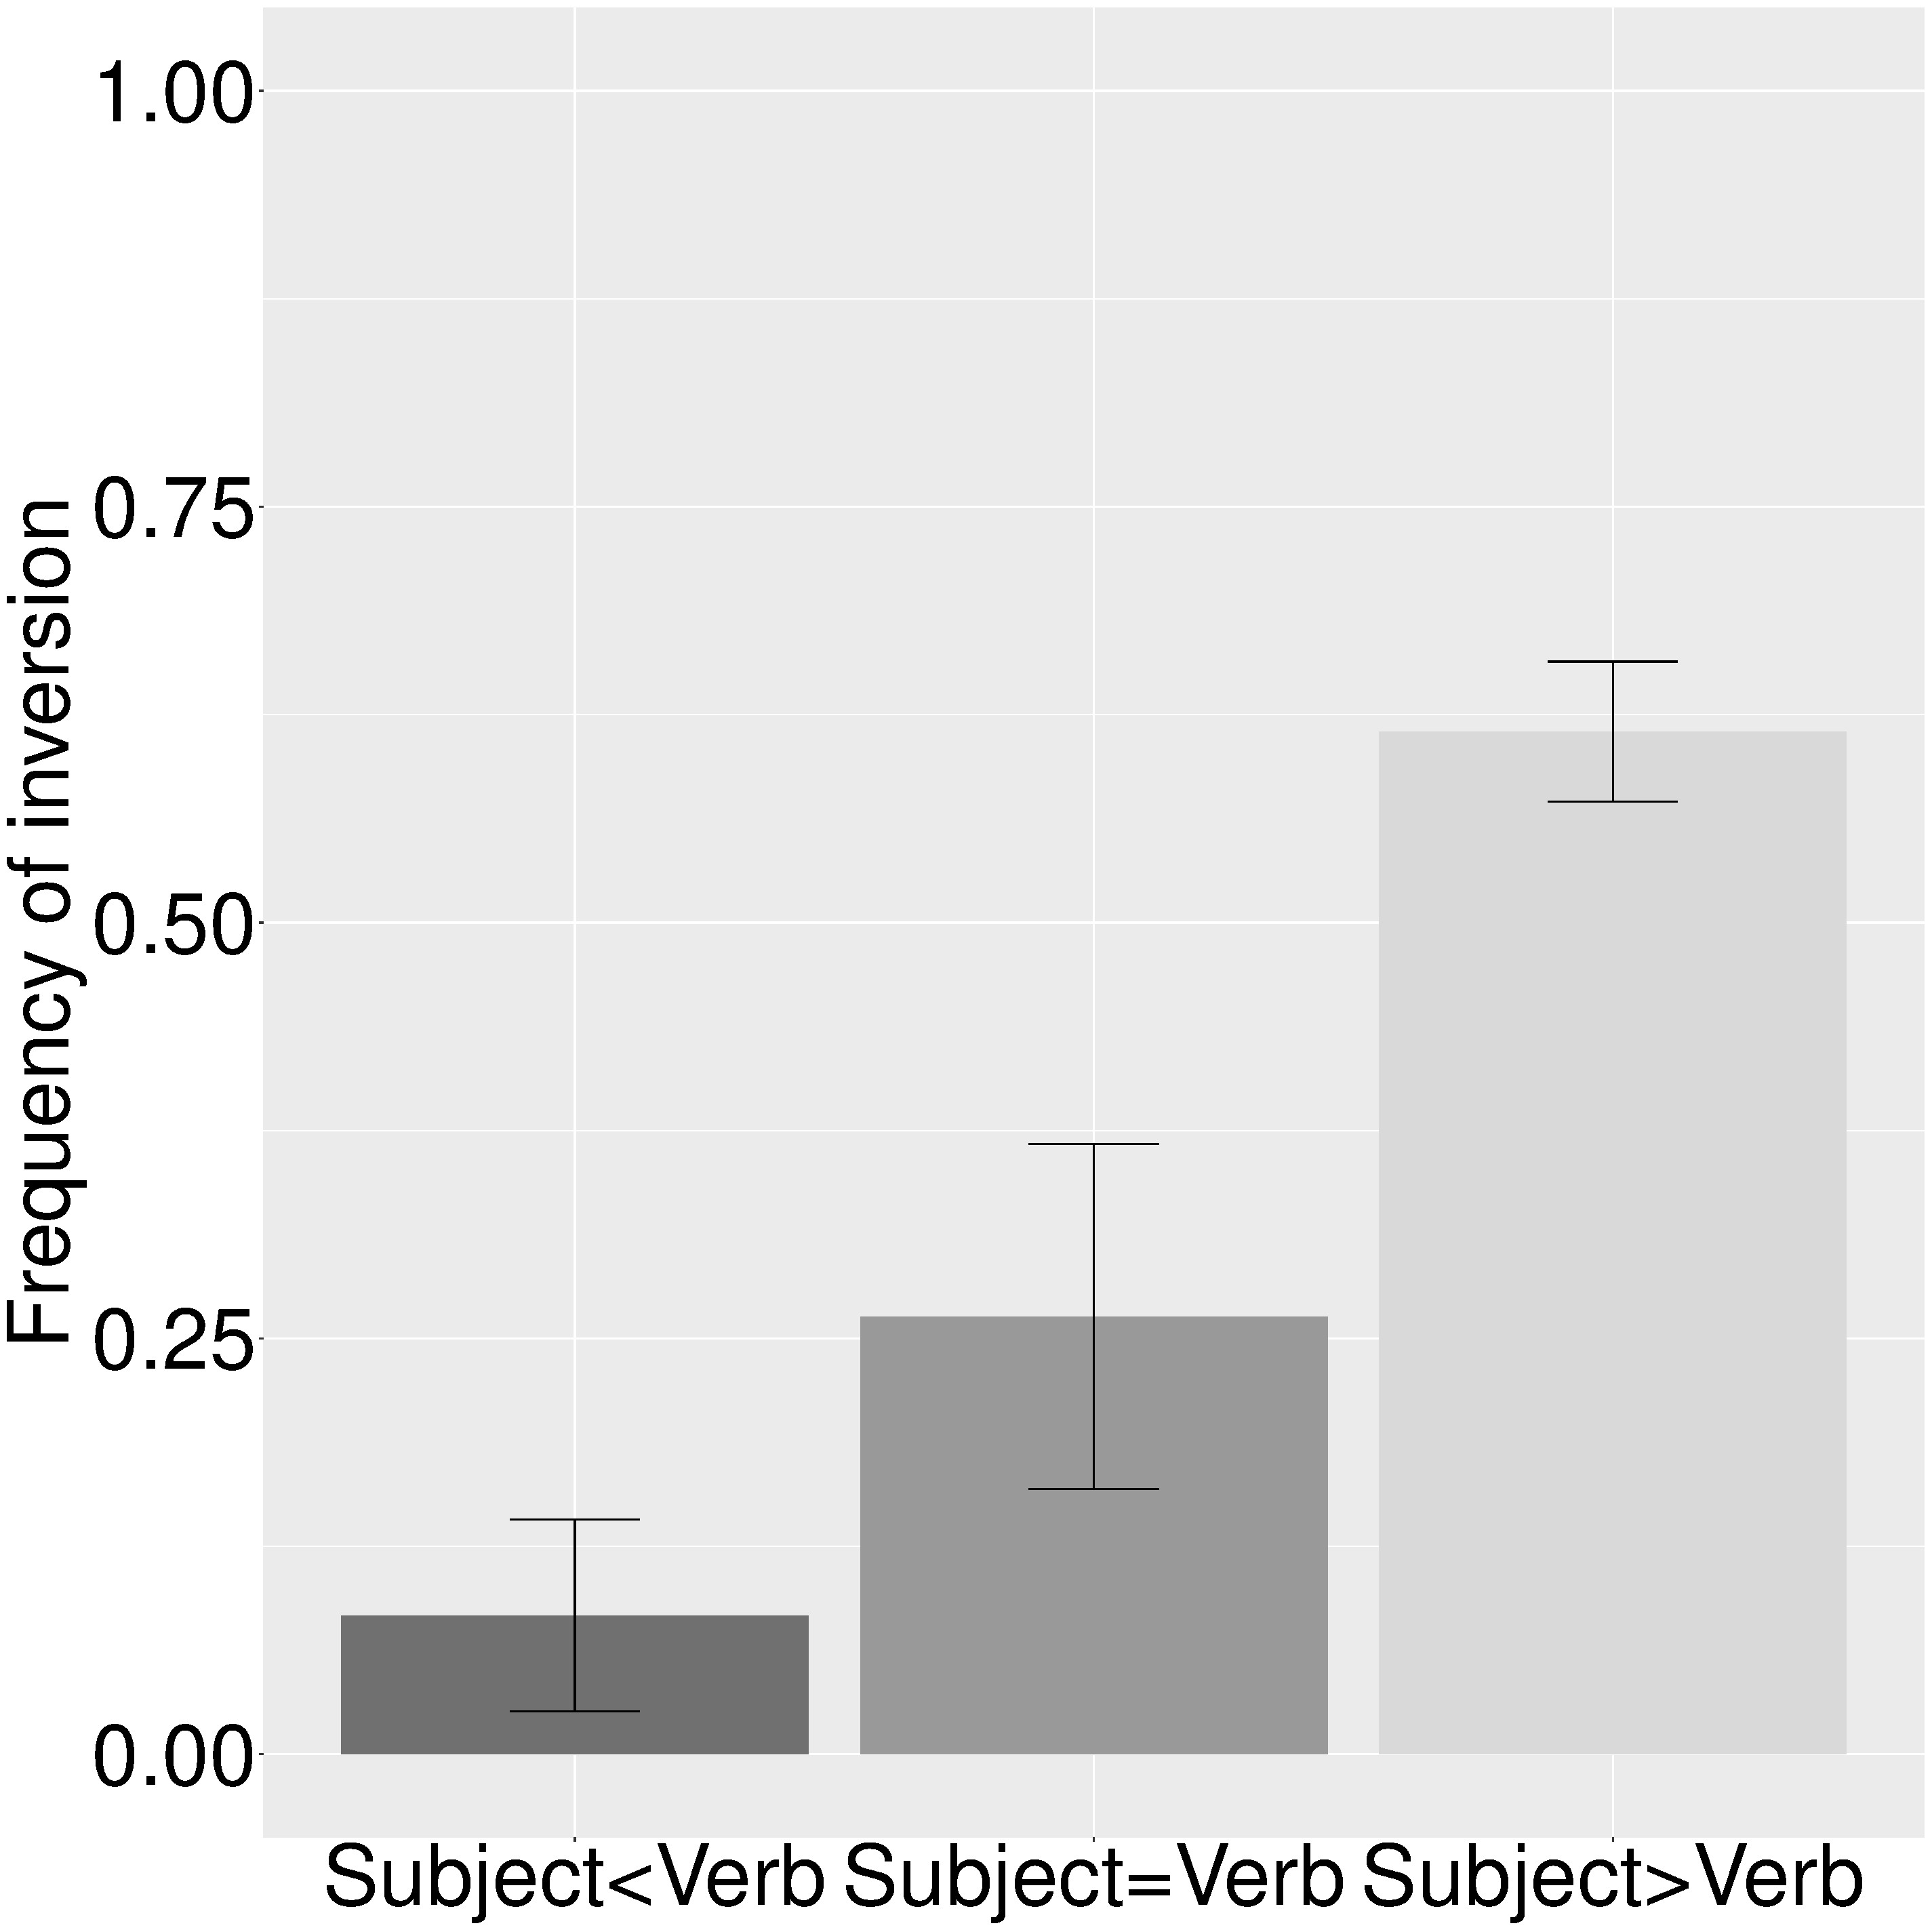
\includegraphics[width = .48\linewidth]{figures/pozhemab3.pdf}}
\subfigure[Object Definiteness]{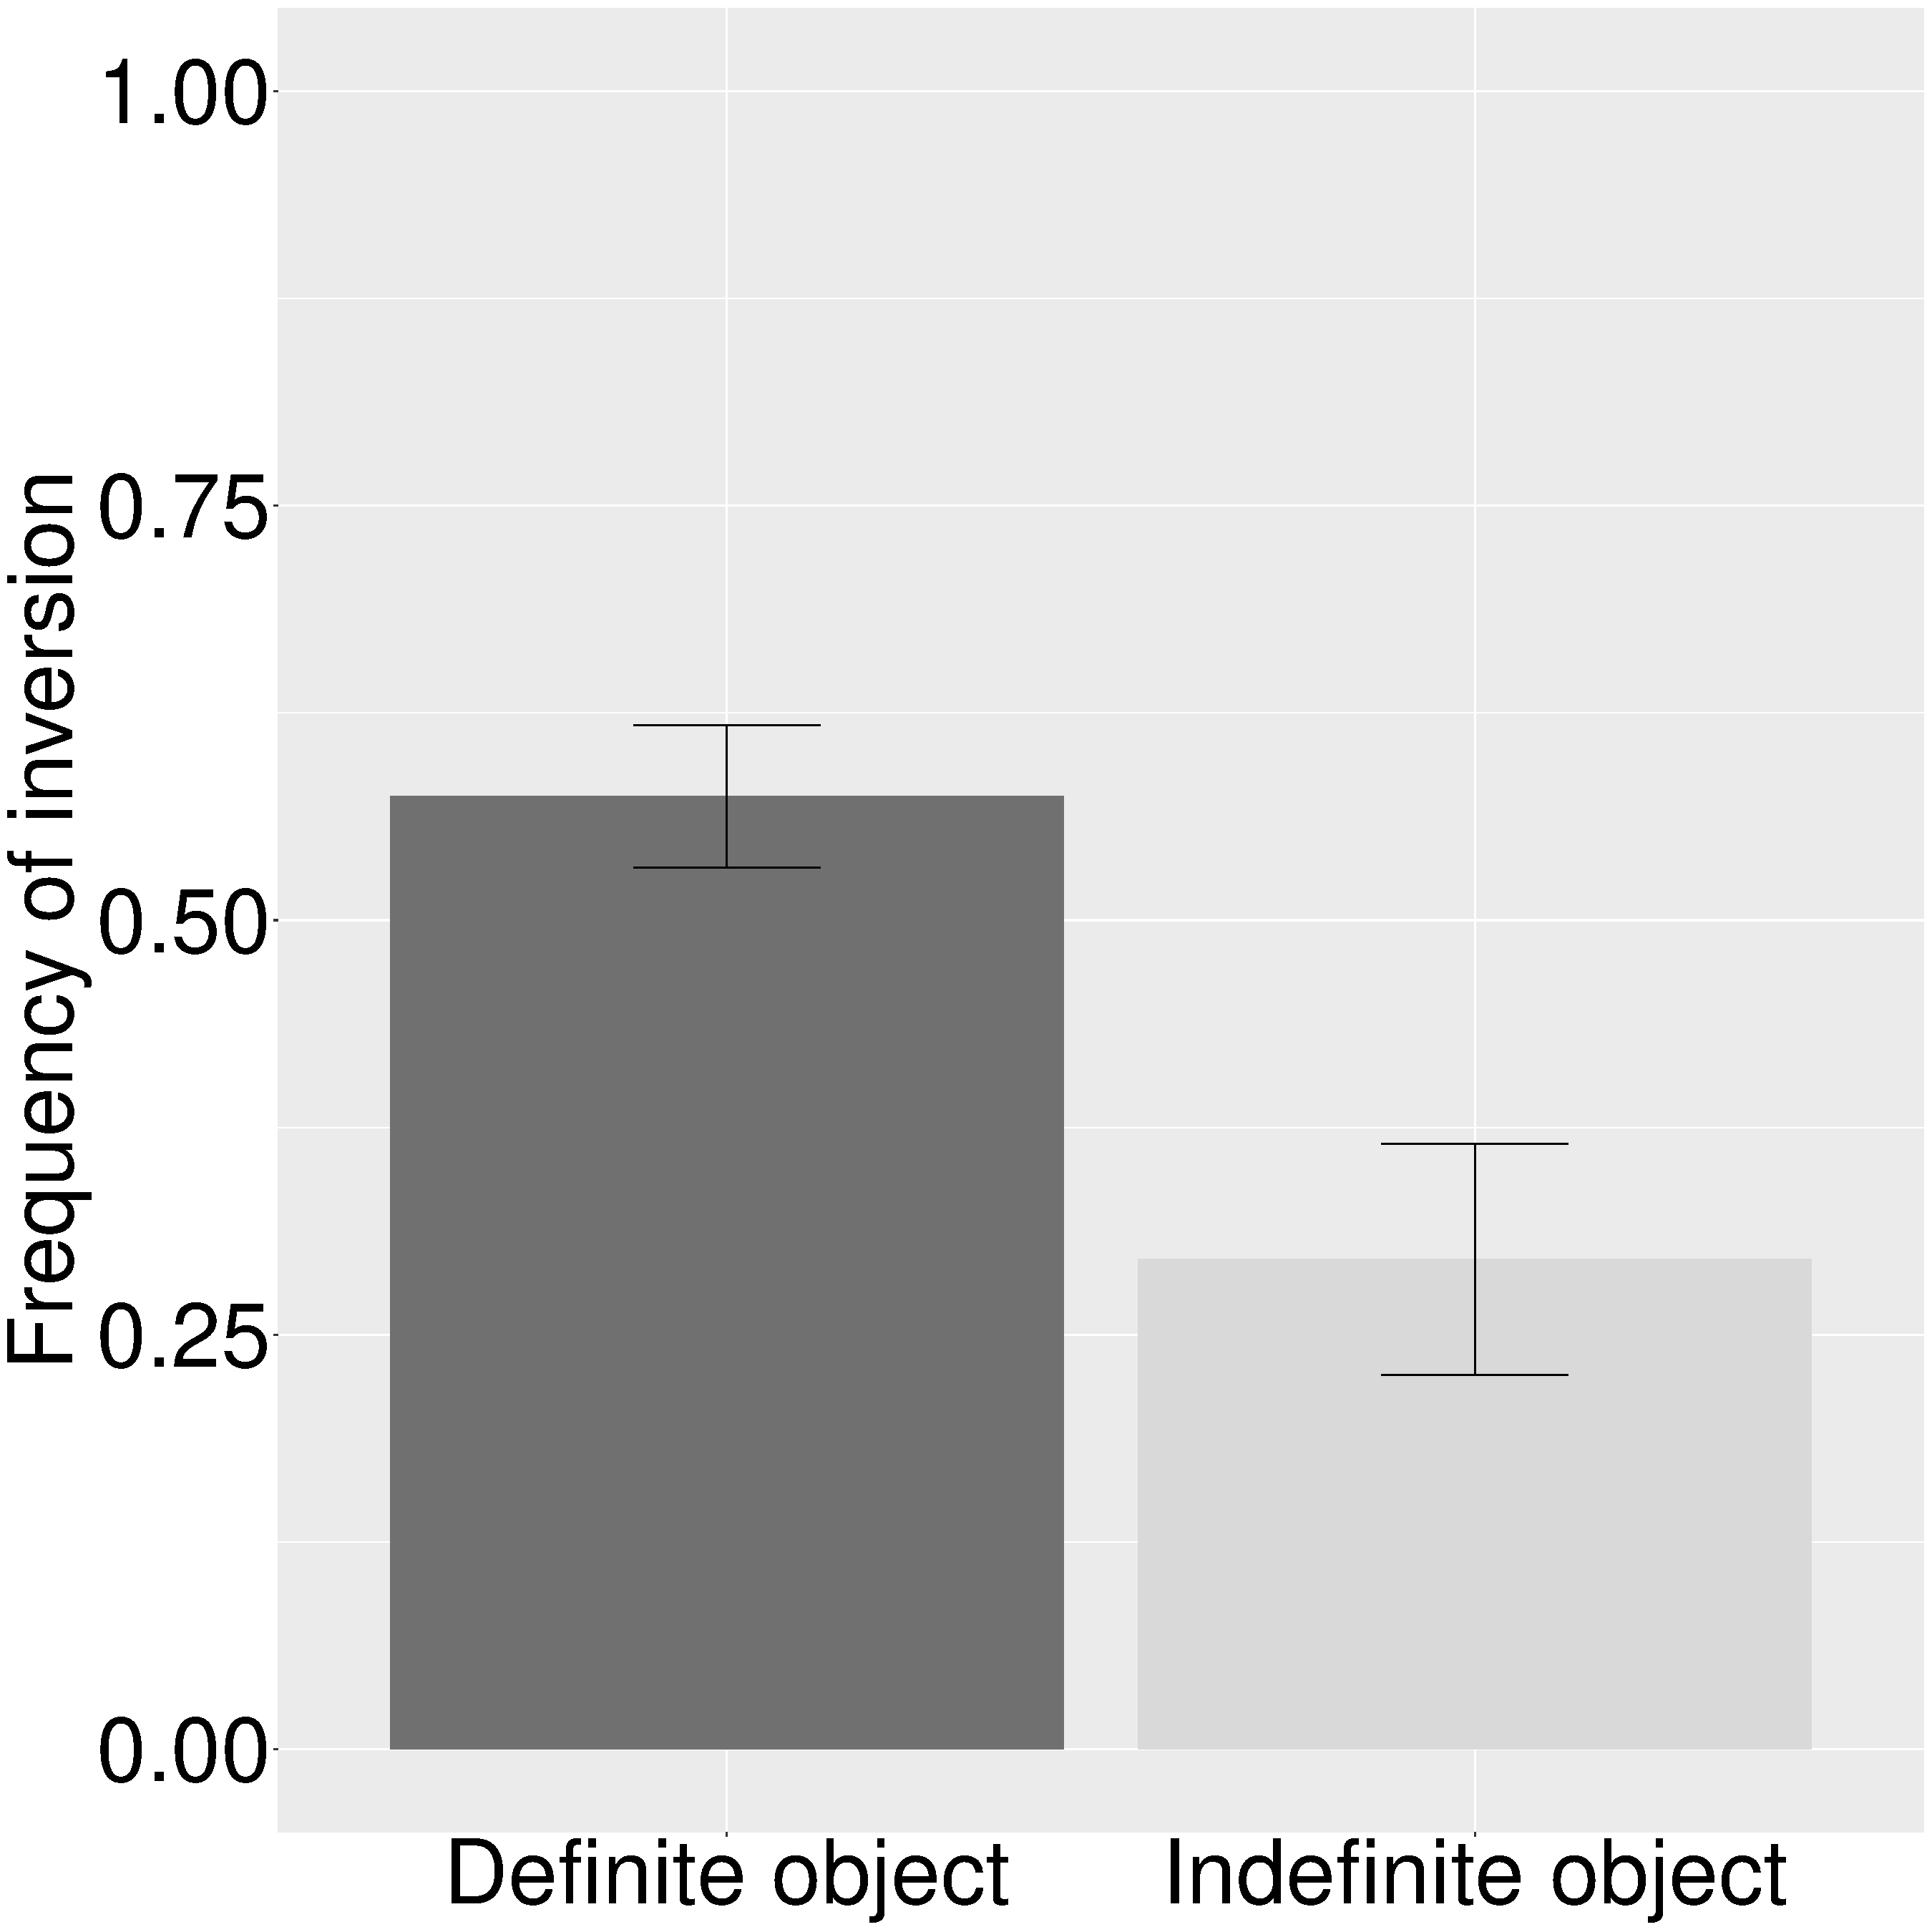
\includegraphics[width = .48\linewidth]{figures/pozhemab4.pdf}}\\
\caption{Significant factors on subject inversion (corpus study)\label{figcorpus}}
\end{figure}

\subsection{Interim discussion}


The corpus study shows that subject inversion can be as frequent as preverbal subjects for object relatives with a nominal subject. It also shows that object relatives with pre- and postverbal subjects have different properties: A preverbal subject is more frequent when the object is indefinite and  the subject intentional (implying agentivity of the verb), and  when the relative is short (including only the subject and the verb) and with a subject that is shorter than the verb.  A postverbal subject is more frequent when it is longer than the verb, when it is non-intentional and has a definite object, and when the relative clause is long. 
The relative length effect (verb shorter than the subject) is in line with processing theories like DLT which predict processing difficulty with a long intervening subject between {\textit{que}} and the verb (or between {\textit{que}} and the postverbal gap), thus favouring subject inversion. It may also be explained by a more general tendency to put longer (heavier) constituents at the end of the sentence  \citep{Behaghel, wasow2002postverbal}. 

Prosodic factors may also play a role in explaining why a short relative (subject and verb only) favours inversion. If one considers the general tendency to have balanced prosodic constituents, and that a prosodic boundary usually occurs between the subject and the verb \citep{di2016}, (\ref{expros1}) has a less natural prosodic structure than (\ref{expros2}) (with a longer relative) or (\ref{expros3}) (with subject inversion).



\begin{exe}
\ex \label{expros1}

\gll les problèmes (que l’audiovisuel) (connaît).\\
the problems that {the audiovisual} knows \\    
\glt ‘the problems that the audiovisual knows…'
\ex \label{expros2}
\gll les problèmes (que l’audiovisuel) (connaît dans la région) \\
the problems that {the audiovisual} knows in the region \\    
\glt ‘the problems that the audiovisual knows in the region’

\ex \label{expros3}
\gll les problèmes (que connaît) (l’audiovisuel) \\
the problems that knows {the audiovisual}\\    
\glt‘the problems that the audiovisual knows’
\end{exe}


The definiteness effect can be explained by the relative discourse
status of the subject and the object: in the context of an object
relative clause, a definite object is more topical than the subject,
and a less topical subject is more likely to be postverbal
\citep{kampers2004}. The effect of subject intentionality or
agentivity of the verb is in line with \citet{marandin2011} and
\citet{Bonami}, suggesting that postverbal subjects lose their dynamic
and agentive properties.
%please check the Bonami and Danièle reference\\

The corpus analysis thus shows that semantic/pragmatic features differ
for object relatives with a preverbal subject and object relatives
with a postverbal subject. Verb semantics, length and definiteness
seem to play an important role, meaning that subject inversion in
object relative clauses is not merely a stylistic variant. However,
corpus studies suffer from the problem that the factors of interest
are often intercorrelated, as we have seen for the intentionality of
the subject and agentivity of the verb. Also, the constraints we
annotated may be affected by some other variables co-varying in the
corpus that we have not taken into account. In order to have a more
controlled picture of the usage difference, we therefore tested these
factors with two experimental studies.


\section{Subject inversion in object relatives: An acceptability judgement task}

In order to better understand the use of object relatives with
preverbal and post\-verbal subjects, we ran an acceptability judgement
task manipulating some of the factors found in the corpus study.

\subsection{Material}


We manipulated three variables: subject position
(preverbal/postverbal), verb semantics (agentive/non-agentive) and
subject length (long/short). As for verb semantics, pairs of agentive
and non-agentive verbs were created with the same number of
syllables. Verb agentivity is highly correlated with subject
intentionality, as we saw in the preceding section, and easier to
control in the experimental materials. Concerning subject length, the
subject was treated as short when it was only composed of the article and the
noun, whereas it was considered as long when a noun complement and/or
an adjective was included.

Thirty-two items were created with four items per condition (Latin
square design), as shown in Table \ref{tab:4:annotation}. Forty-four
fillers were added as distractors. The subject was always animate
(humans, human groups or nouns symbolizing a collective group like a
firm or a country) and the object inanimate, which favors object
relative processing across the two variants \citep{Frauenfelder1980,
  mak2006animacy}. The experimental materials were inspired by the
sentences from the corpus study. All relatives were short
(relativizer, subject, verb), the object and the subject were
definite, and all relatives modified the main clause subject. Subject
length was manipulated by adding a modifier or a complement to the
subject noun; the agentivity condition was an alternation between two
related verbs, one non-agentive like {\textit{cost}} making the
subject non-intentional, and one agentive like \textit{pay} making the
subject intentional.\footnote{The materials and the entire analysis
  can be found on \url{https://osf.io/k97pu/}.}



\begin{sidewaystable}
\small
  \begin{tabular}{cccl} 
   \lsptoprule
 Inv & Ag & Long & Example\\
   \midrule
 $-$ & $-$ &  $-$  & Le prix astronomique que la firme coûte énerve considérablement les dirigeants. \\
 & & & the price astronomical that the company costs irritates considerably the managers \\
 & & & `The astronomical price that the company costs considerably irritates the managers.' \\
$+$ & $-$ &  $-$  &	Le prix astronomique que coûte la firme énerve considérablement les dirigeants. \\
& & & the price astronomical that costs the company irritates considerably the managers \\
& & & `The astronomical price that the company costs considerably irritates the managers.' \\
$-$ & $-$ &  $+$  & 	Le prix astronomique que la firme agroalimentaire coûte énerve considérablement les dirigeants. \\
& & & the price astronomical that the company agri-food  costs irritates considerably the managers \\
& & & `The astronomical price that the agri-food company costs considerably irritates the managers.'\\
$+$ & $-$ &  $+$  &	Le prix astronomique que coûte la firme agroalimentaire énerve considérablement les dirigeants.\\
& & & the price astronomical that costs the company agri-food irritates considerably the managers \\
& & & `The astronomical price that the agri-food company costs considerably irritates the managers.'\\
$-$ & $+$ & $-$  &	Le prix astronomique que la firme paie énerve considérablement les dirigeants.\\
& & & the price astronomical that the company pays irritates considerably the managers \\
& & & `The astronomical price that the company pays considerably irritates the managers.' \\
$+$ & $+$ & $-$   &	Le prix astronomique que paie la firme énerve considérablement les dirigeants.\\
& & & the price astronomical that pays the company pays irritates considerably the managers \\
& & & `The astronomical price that  the company pays considerably irritates the managers.'\\
$-$ & $+$ & $+$  &	Le prix astronomique que la firme agroalimentaire paie énerve considérablement les dirigeants.\\
& & & the price astronomical that the company agri-food  pays irritates considerably the managers \\
& & & `The astronomical price that the agri-food company pays considerably irritates the managers.'\\
 $+$ & $+$ & $+$  &	Le prix astronomique que paie la firme agroalimentaire énerve considérablement les dirigeants.\\
& & & the price astronomical that pays the company agri-food irritates considerably the managers \\
& & & `The astronomical price that  the agri-food company pays considerably irritates the managers.'\\
  \lspbottomrule
 \end{tabular}
% \resizebox{\columnwidth}{!}{%
%  \begin{tabular}{ll l} 
 
%   \lsptoprule
%   Condition 1 & Non-inversion/non-agentive/Short subject &	Le prix astronomique que la firme coûte énerve considérablement les dirigeants. \\
% & & The price astronomical that the company costs irritates considerably the managers. \\
%  & & `The astronomical price that the company costs considerably irritates the managers.' \\
% Condition 2 &
% Inversion/Non-agentive/Short subject &	Le prix astronomique que coûte la firme énerve considérablement les dirigeants. \\
% & & The price astronomical that costs the company irritates considerably the managers. \\
% & & `The astronomical price that the company costs considerably irritates the managers.' \\
% Condition 3 &
% Non-inversion/Non-agentive/Long subject & 	Le prix astronomique que la firme agroalimentaire coûte énerve considérablement les dirigeants. \\
% & & The price astronomical that the company agri-food  costs irritates considerably the managers. \\
% & & `The astronomical price that the agri-food company costs considerably irritates the managers.'\\
% Condition 4 &
%  Inversion/Non-agentive/Long subject &	Le prix astronomique que coûte la firme agroalimentaire énerve considérablement les dirigeants.\\
%  & & The price astronomical that costs the company agri-food irritates considerably the managers. \\
% & & `The astronomical price that the agri-food company costs considerably irritates the managers.'\\
% Condition 5 &
% Non-inversion/Agentive/Short subject &	Le prix astronomique que la firme paie énerve considérablement les dirigeants.\\
% & & The price astronomical that the company pays irritates considerably the managers. \\
% & &` The astronomical price that the company pays considerably irritates the managers.' \\
% Condition 6 &
% Inversion/Agentive/Short subject  &	Le prix astronomique que paie la firme énerve considérablement les dirigeants.\\
% & & The price astronomical that pays the company pays irritates considerably the managers. \\
% & & `The astronomical price that  the company pays considerably irritates the managers.'\\
% Condition 7 &
% Non-inversion/Agentive/Long subject &	Le prix astronomique que la firme agroalimentaire paie énerve considérablement les dirigeants.\\
% & & The price astronomical that the company agri-food  pays irritates considerably the managers. \\
% & & `The astronomical price that the agri-food company pays considerably irritates the managers.'\\
% Condition 8 &
%  Inversion/Agentive/Long subject &	Le prix astronomique que paie la firme agroalimentaire énerve considérablement les dirigeants.\\
%  & & The price astronomical that pays the company agri-food irritates considerably the managers. \\
% & & `The astronomical price that  the agri-food company pays considerably irritates the managers.'\\

%   \lspbottomrule
%  \end{tabular}%
%  }
 \caption{Examples of sentences used in the acceptability judgement
   task:  subject inversion (Inv ±), verb agentivity (Ag ±), subject length (Long ±) 
   \label{tab:4:annotation}}
\end{sidewaystable}


\subsection{Participants}
Eighty French native speakers (56 women, mean age: 36 years, $\sigma=18$) volunteered to participate in the experiment, which was run on IbexFarm \citep{drummond2013ibex}. They were recruited via the RISC (\url{http://www.risc.cnrs.fr}) platform. 

\subsection{Procedure}
Participants read sentences on a computer screen at a location of their choice. They had to judge the acceptability of each sentence on a scale from 1 (not at all acceptable) to 10 (fully acceptable). The experiment lasted about 15 minutes.

\subsection{Results}
We analyzed the acceptability judgements with generalized linear mixed models \citep{baayen2008mixed}, using the \texttt{lmer} function in R with the \texttt{lme4} package from \citet{Bates2015}. As predictors, we included subject length (short, long), verb semantics (agentive, non-agentive) and subject position (postverbal, preverbal). We applied mean centered coding for all predictors. Acceptability judgements are the dependent variable in the model. Participants and items were included as random variables. We used a ``maximal model'', by including by-participants and by-items random intercepts as well as random slopes for all the relevant fixed factors \citep{barr2013}. We enforced zero correlations between random effects in order to avoid overparameterization or false convergence \citep{Bates2015}.  Figure \ref{figure3judgementresults} illustrates the effects of the three independent variables on judgements. 

\begin{figure}
\subfigure[Verb Agentivity (Ag ±)]{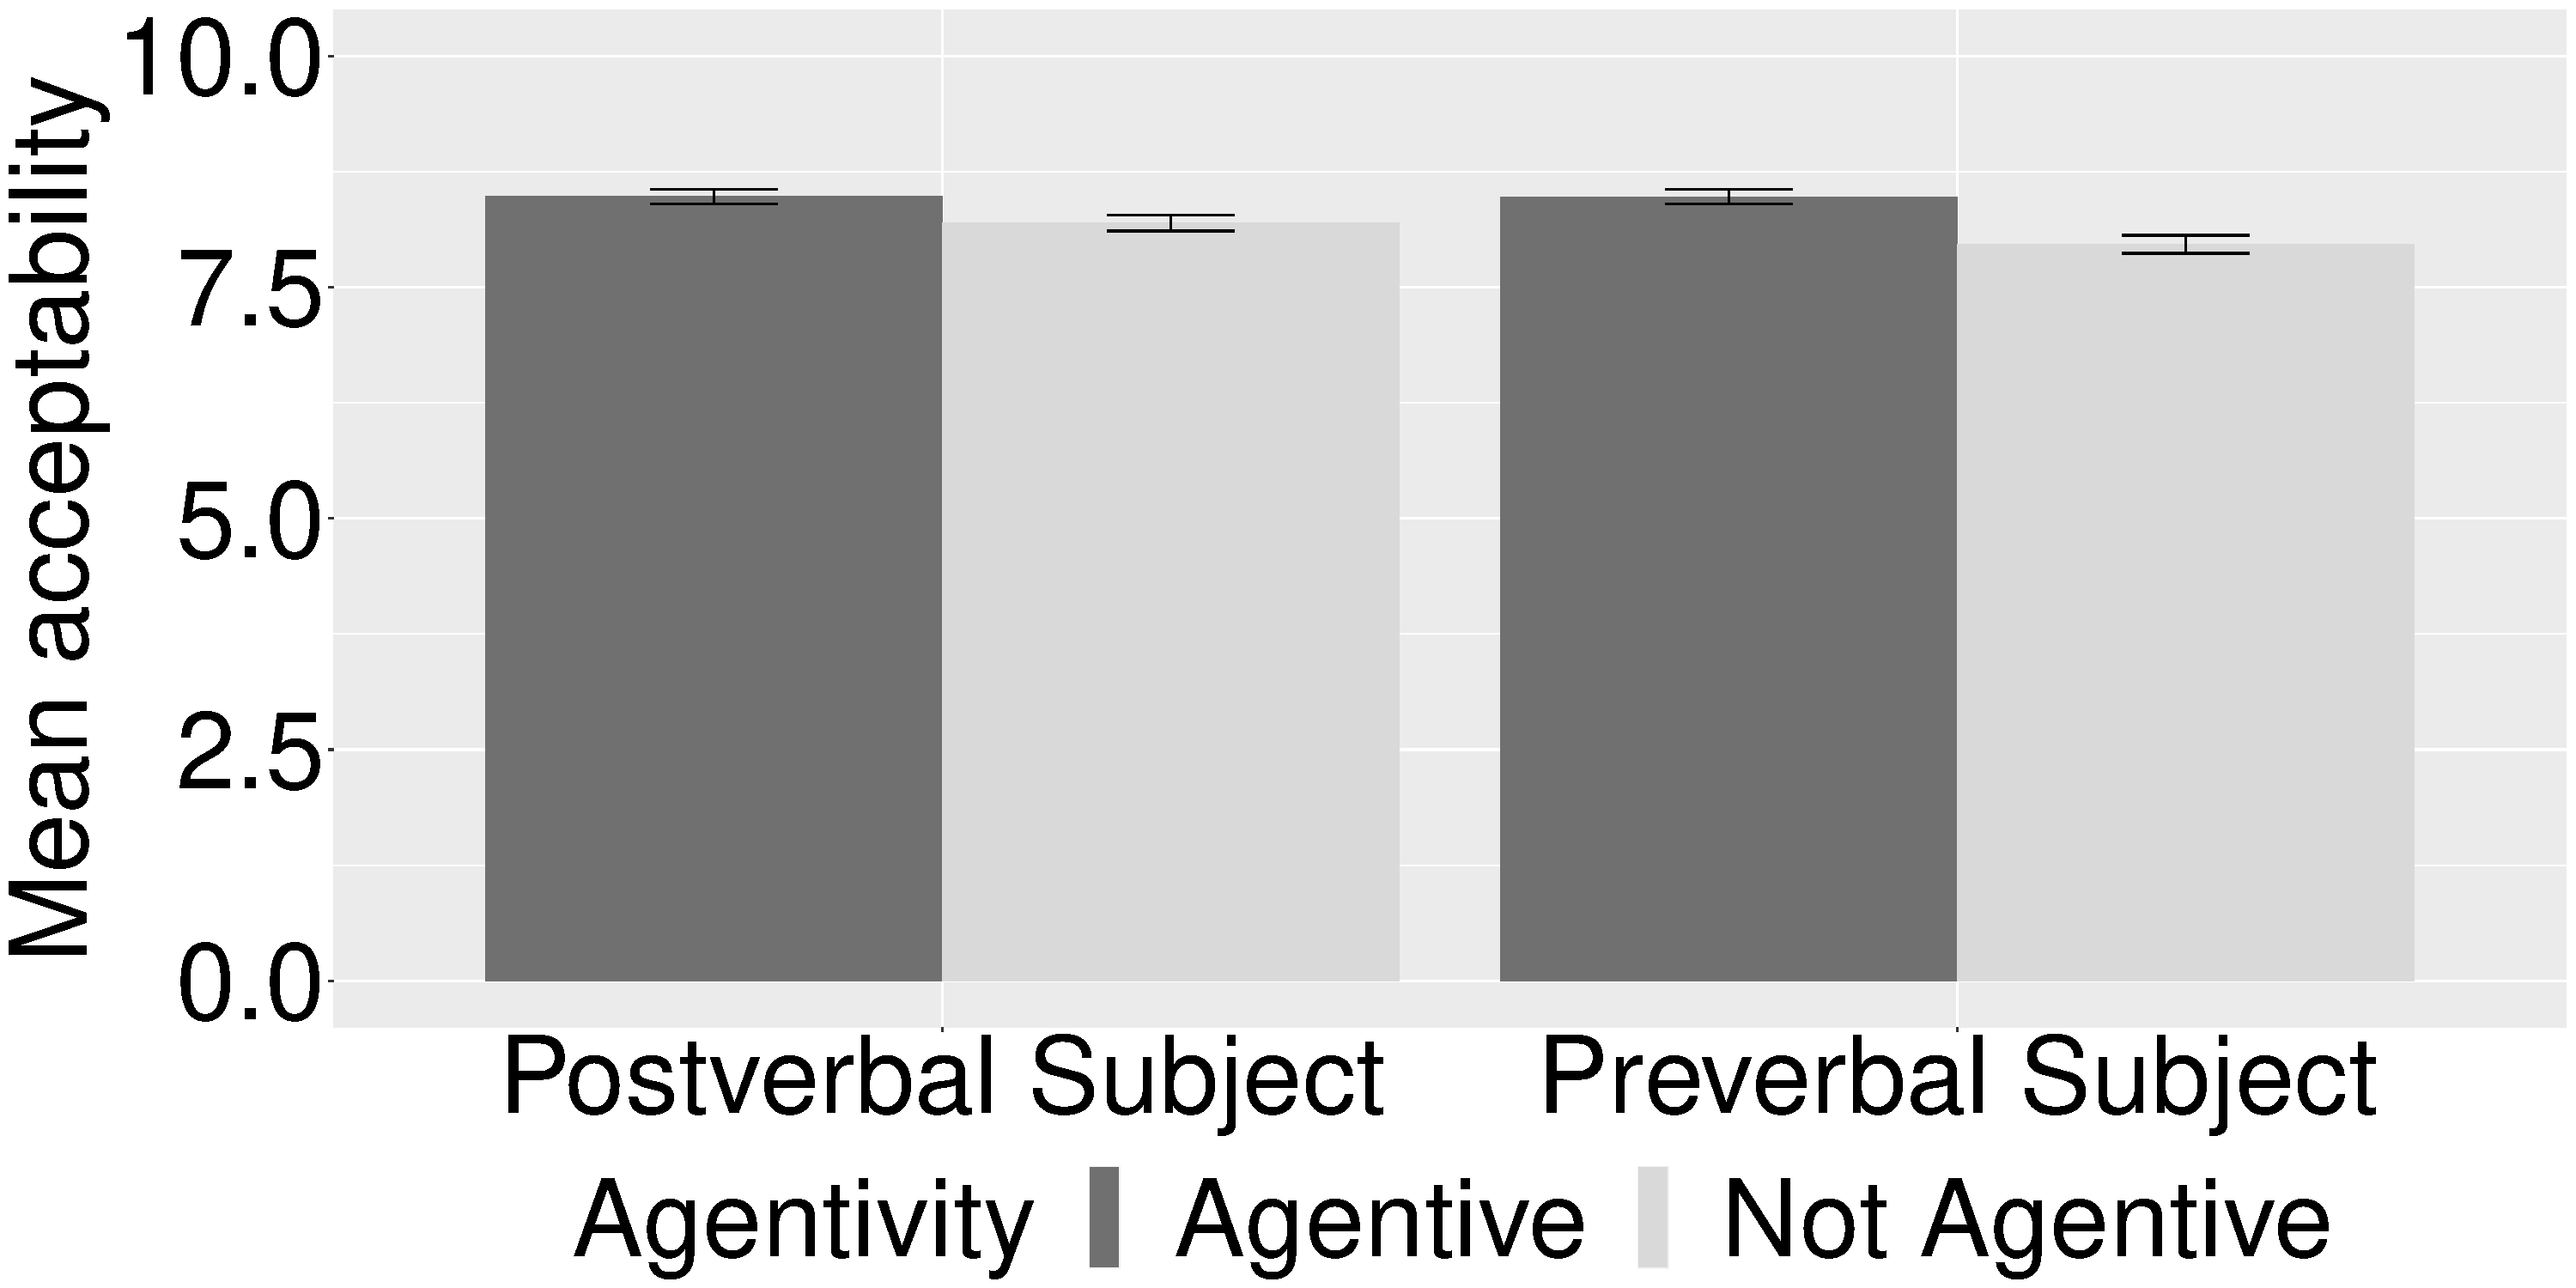
\includegraphics[width = 2.4in]{figures/PozHemAb31.pdf}}
\subfigure[Subject Length (Long ±)]{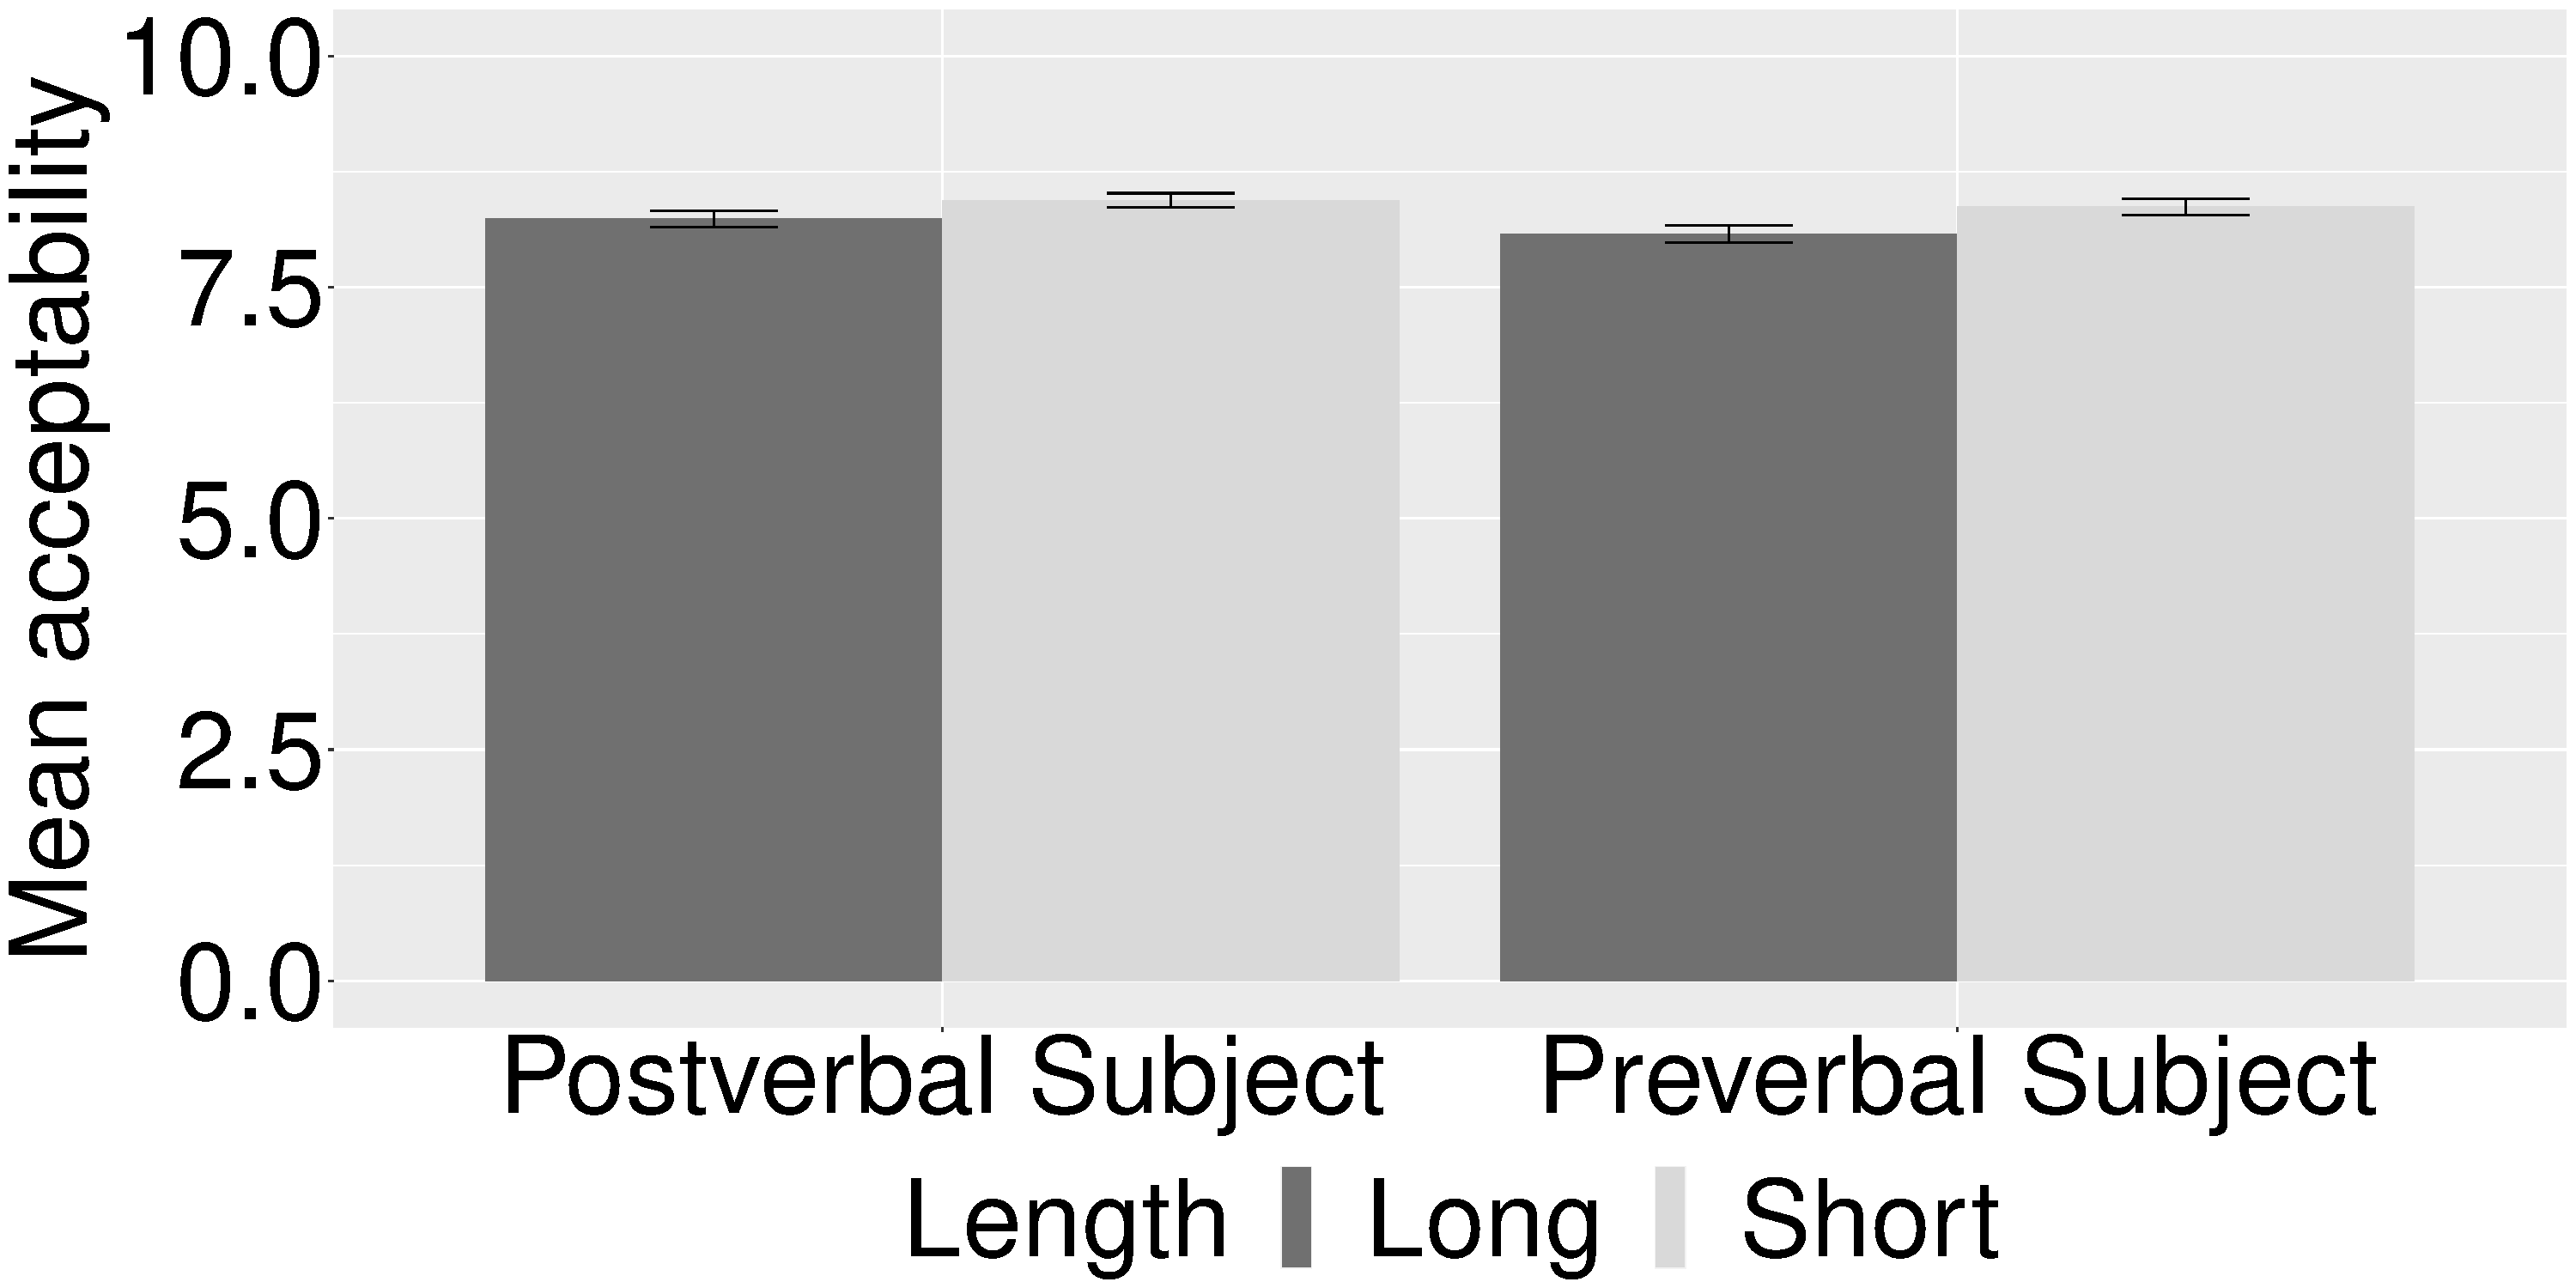
\includegraphics[width = 2.4in]{figures/PozHemAb32.pdf}}
\subfigure[Subject Inversion (Inv ±)]{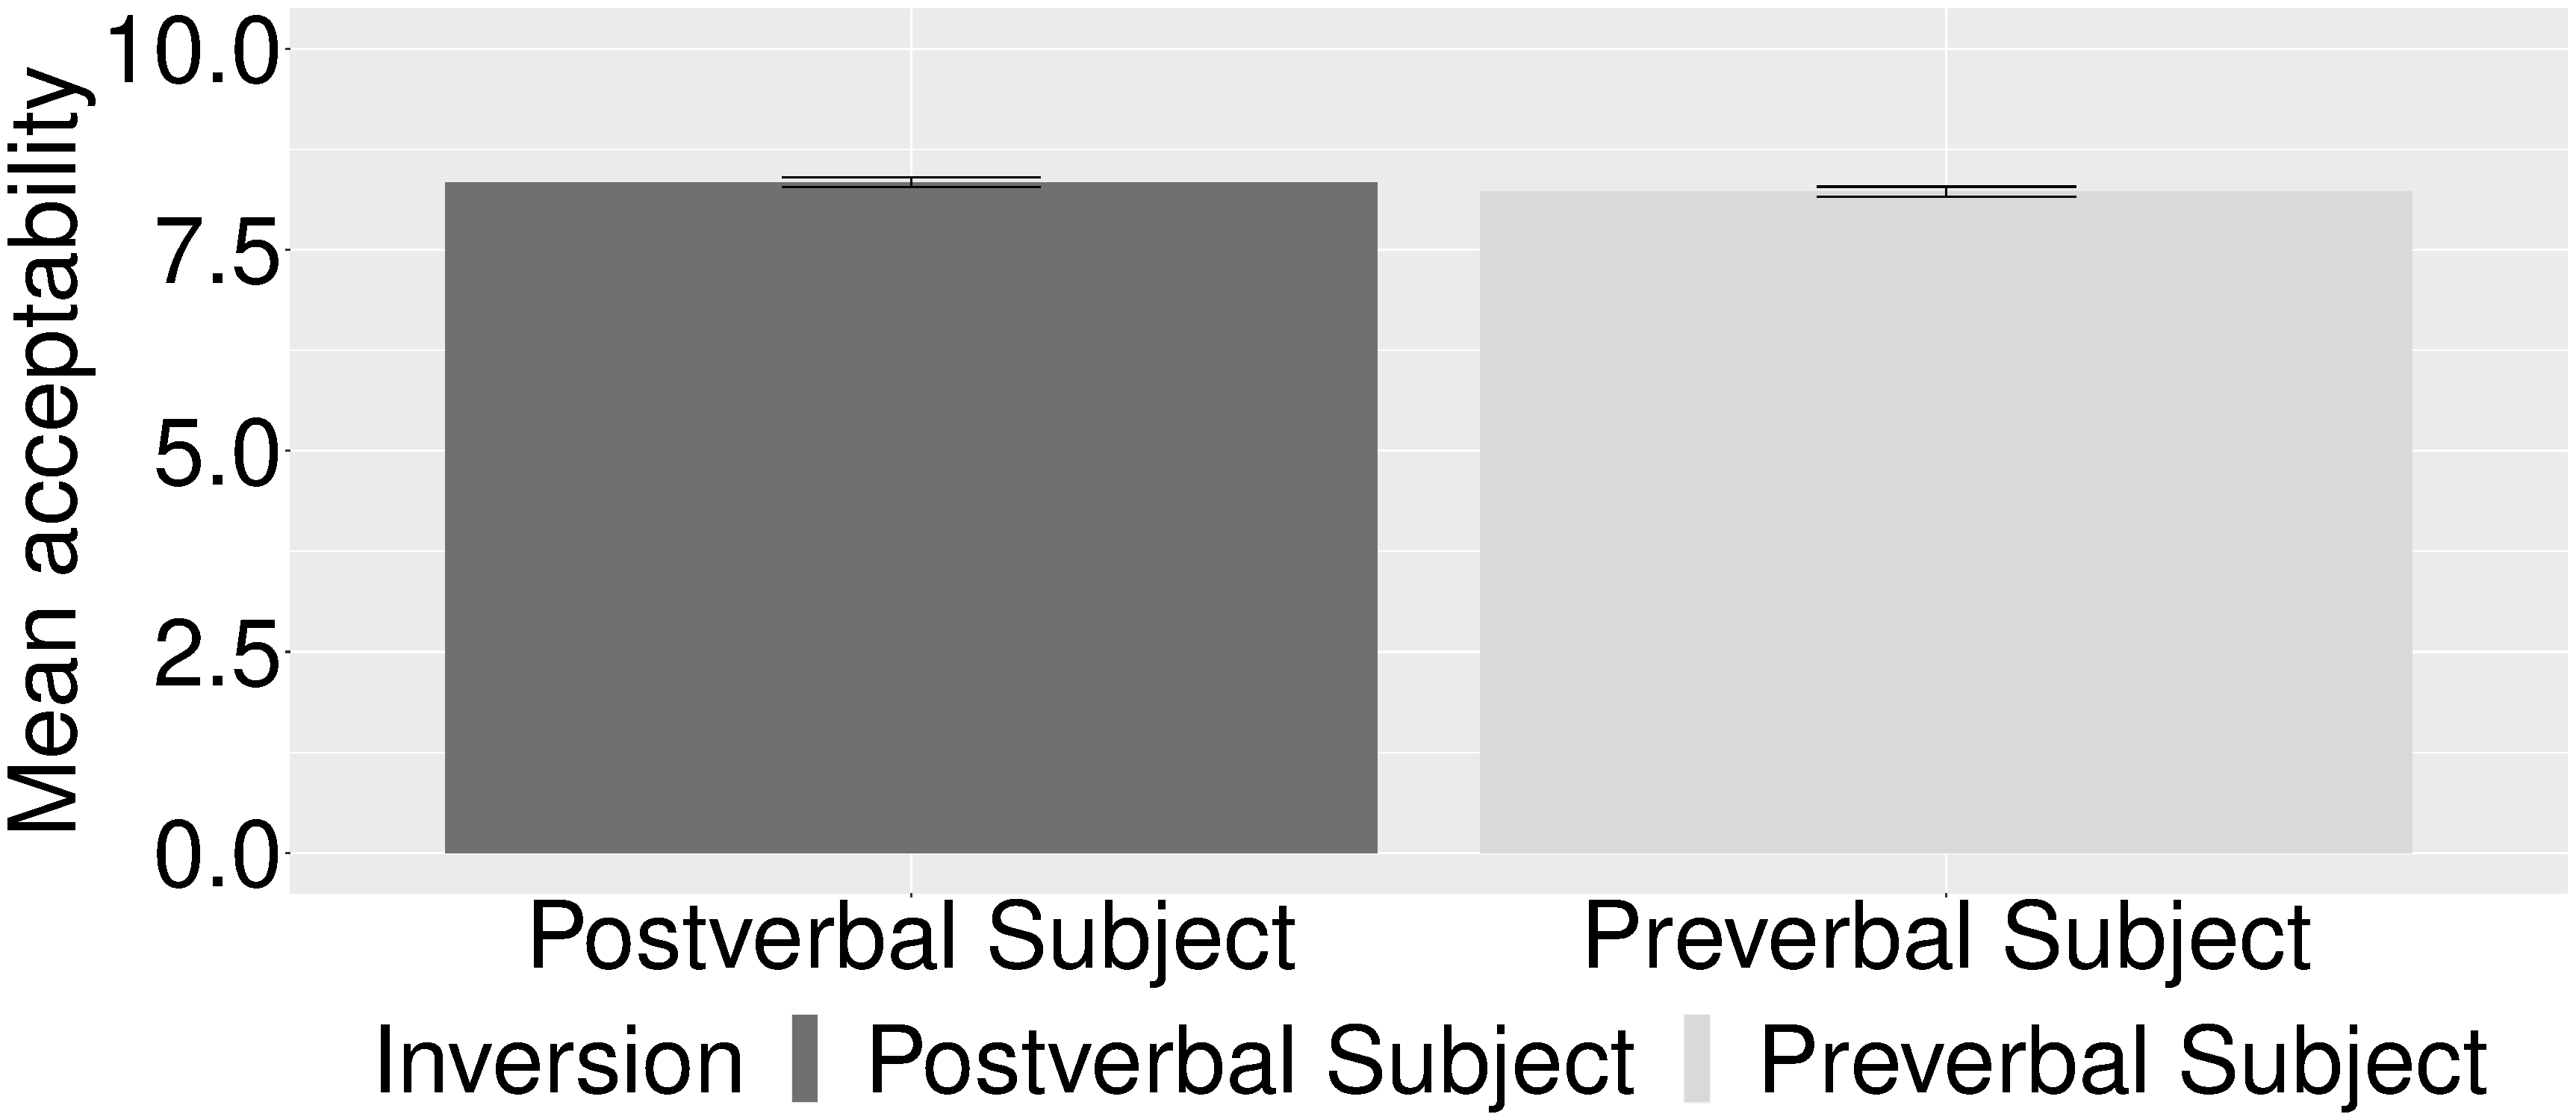
\includegraphics[width = 2.4in]{figures/PozHemAb33.pdf}}
\caption{Influence of verb agentivity, subject length and subject
  inversion on acceptability\label{figure3judgementresults}}
\end{figure}


When looking at subject position, the model shows that relatives both with and without inversion are rated well (higher than 8/10). Object relatives with postverbal subject are considered marginally more acceptable than object relatives with preverbal subject (8.34 vs. 8.22, $t=1.751, p=0.08$).

Main effects of agentivity ($t=2.925, p<0.01$) and subject length ($t=3.322,\allowbreak p<0.01$) were found, meaning that sentences are rated better when the verb is agentive and the subject short. We also found an interaction between those two variables ($t=-2.571, p<0.05$): sentences with short subjects received higher ratings when the verb is not agentive. Otherwise, no significant interaction between the three factors was found. 


\subsection{Interim discussion}
The acceptability judgements showed that relatives both with preverbal subject and with postverbal subject are well acceptable, which is in line with what was found in the corpus study (the two possibilities were used about equally often). The results showed that object relatives with postverbal subject are in fact judged slightly better, contrary to the results from previous experiments \citep{Holmes1981, pozniak2015processing}, which only considered ORs with animate objects and reversible verbs. This can be explained by the fact that all objects were definite in our material and all relatives were short, meaning that, as shown in the corpus study, all our materials already realized two of the constraints that make object relatives with postverbal subject favored, compared to object relatives with preverbal subject.

No interaction was found, however, between subject position, agentivity, and subject length. One reason for this lack of an effect could be that both relatives are perfectly grammatical and that participants chose a rather conscious and metalinguistic approach to the task, which may have obscured subtle differences between object relatives with preverbal subject and object relatives with postverbal subject. In order to have a more fine-grained analysis of processing at every point in the sentence as well as more spontaneous data, we decided to run a self-paced reading experiment with the same material. 

\section{Subject inversion in object relatives: A self-paced reading experiment}\largerpage[2]

Our acceptability judgement task only showed global acceptability ratings of object relatives with preverbal and postverbal subject. This paradigm cannot differentiate which part of the sentence makes a relative clause more or less acceptable and natural. That is why we ran a self-paced reading experiment as well. 

\subsection{Material}
The items used were the same as in the acceptability study and the conditions were the same as well. 16 fillers were added, as well as 24 comprehension questions: 14 questions for experimental items and 10 for fillers, around 50\% of all the trials. 

\subsection{Participants}
Forty-nine French native speakers (36 women, mean age: 29 years, $\sigma=10$) participated online in the experiment via the IbexFarm platform. They were recruited on the RISC platform.

\subsection{Procedure}
Participants read sentences on a computer screen at a place of their choice. Sentences appeared one word at a time in a moving window paradigm (participants had to press the spacebar each time to make the following word appear). After reading each sentence, they had to judge its acceptability on a scale from 1 (not at all acceptable) to 10 (fully acceptable). They had to answer a question about the previous sentence in around 50\% of the trials. The experiment lasted about 15 minutes.


\subsection{Results}\largerpage[2]
Results were analyzed with generalized linear mixed models using the lmer function. Independent variables were again subject length, verb semantics, and subject position, with mean centered coding applied for all predictors. Random variables were participants and items. The dependent variable was the mean reading time on every region of the sentence. Models take into account log-transforma\-tions of reading times as well as general length. 

Again, we used a ``maximal model'', by including by-participants and by-items random intercepts as well as random slopes for all the relevant fixed factors \citep{barr2013}. We enforced zero correlations between random effects in order to avoid overparameterization or false convergence \citep{Bates2015}.\footnote{The entire analysis can be found on \url{https://osf.io/k97pu/}.} 

\subsubsection{Comprehension questions}
The percentage of correct answers to comprehension questions was above 90\% in all eight conditions. Logistic regression models do not show a significant difference between the conditions.

\subsubsection{Mean reading times}
For the statistical analysis, we divided the items into six regions of interest: antecedent of the relative (object), relativizer, subject/verb, verb/subject, main clause verb, end of the sentence. This is illustrated in Table \ref{tab:5} for conditions without subject inversion and in Table \ref{tab:6} with subject inversion. Figure \ref{figureselfpacedallresults} represents the results for all regions and all conditions. 


\begin{table}
%  \begin{tabular}{llllll} 
%  \lsptoprule
%   1 &	2 &	3 &	4 &	5 &	6 \\
%    \midrule
%    Le prix astronomique    &	que	 & la firme (agroalimentaire) &	coûte/paie &	irrite &	considérablement les dirigeants. \\
%    The  price astronomical &	that &	the  company  (agrifood) &	costs/pays &	irritates &	considerably the managers. \\
%   \lspbottomrule
%  \end{tabular}
 \begin{tabular}{lll}
 \lsptoprule
 1 & Le prix astronomique  & The  price astronomical\\     
 2 & que & that \\    
 3 & la firme (agroalimentaire) & the  company  (agrifood)\\
 4 & coûte/paie & costs/pays\\                                                      
 5 & irrite & irritates\\                                                                        
 6 & considérablement les dirigeants. & considerably the managers. \\                                                                                      
 \lspbottomrule
 \end{tabular}
 \caption{Regions without subject inversion\label{tab:5}}
\end{table}


\begin{table}
%  \begin{tabular}{llllll} 
%  \lsptoprule
%   1 &	2 &	3 &	4 &	5 &	6 \\
%    \midrule
% Le prix astronomique &	que	    &	coûte/paie  &la firme (agroalimentaire) &	irrite &	considérablement les dirigeants. \\
% The  price astronomical &	that &	costs/pays  &	the company (agrifood)  &	irritates &	considerably the managers. \\
% \lspbottomrule
%  \end{tabular} 
 \begin{tabular}{lll}
 \lsptoprule
 1 & Le prix astronomique & The  price astronomical\\ 
 2 & que & that\\                     
 3 & coûte/paie & costs/pays\\                                           
 4 & la firme (agroalimentaire) & the company (agrifood) \\                              
 5 & irrite & irritates\\                               
 6 & considérablement les dirigeants. & considerably the managers.\\                                                                
 \lspbottomrule                                                        
 \end{tabular}
 \caption{Regions with subject inversion\label{tab:6}}
\end{table}


%% format pdf and delete e in posteverbal

\begin{figure}
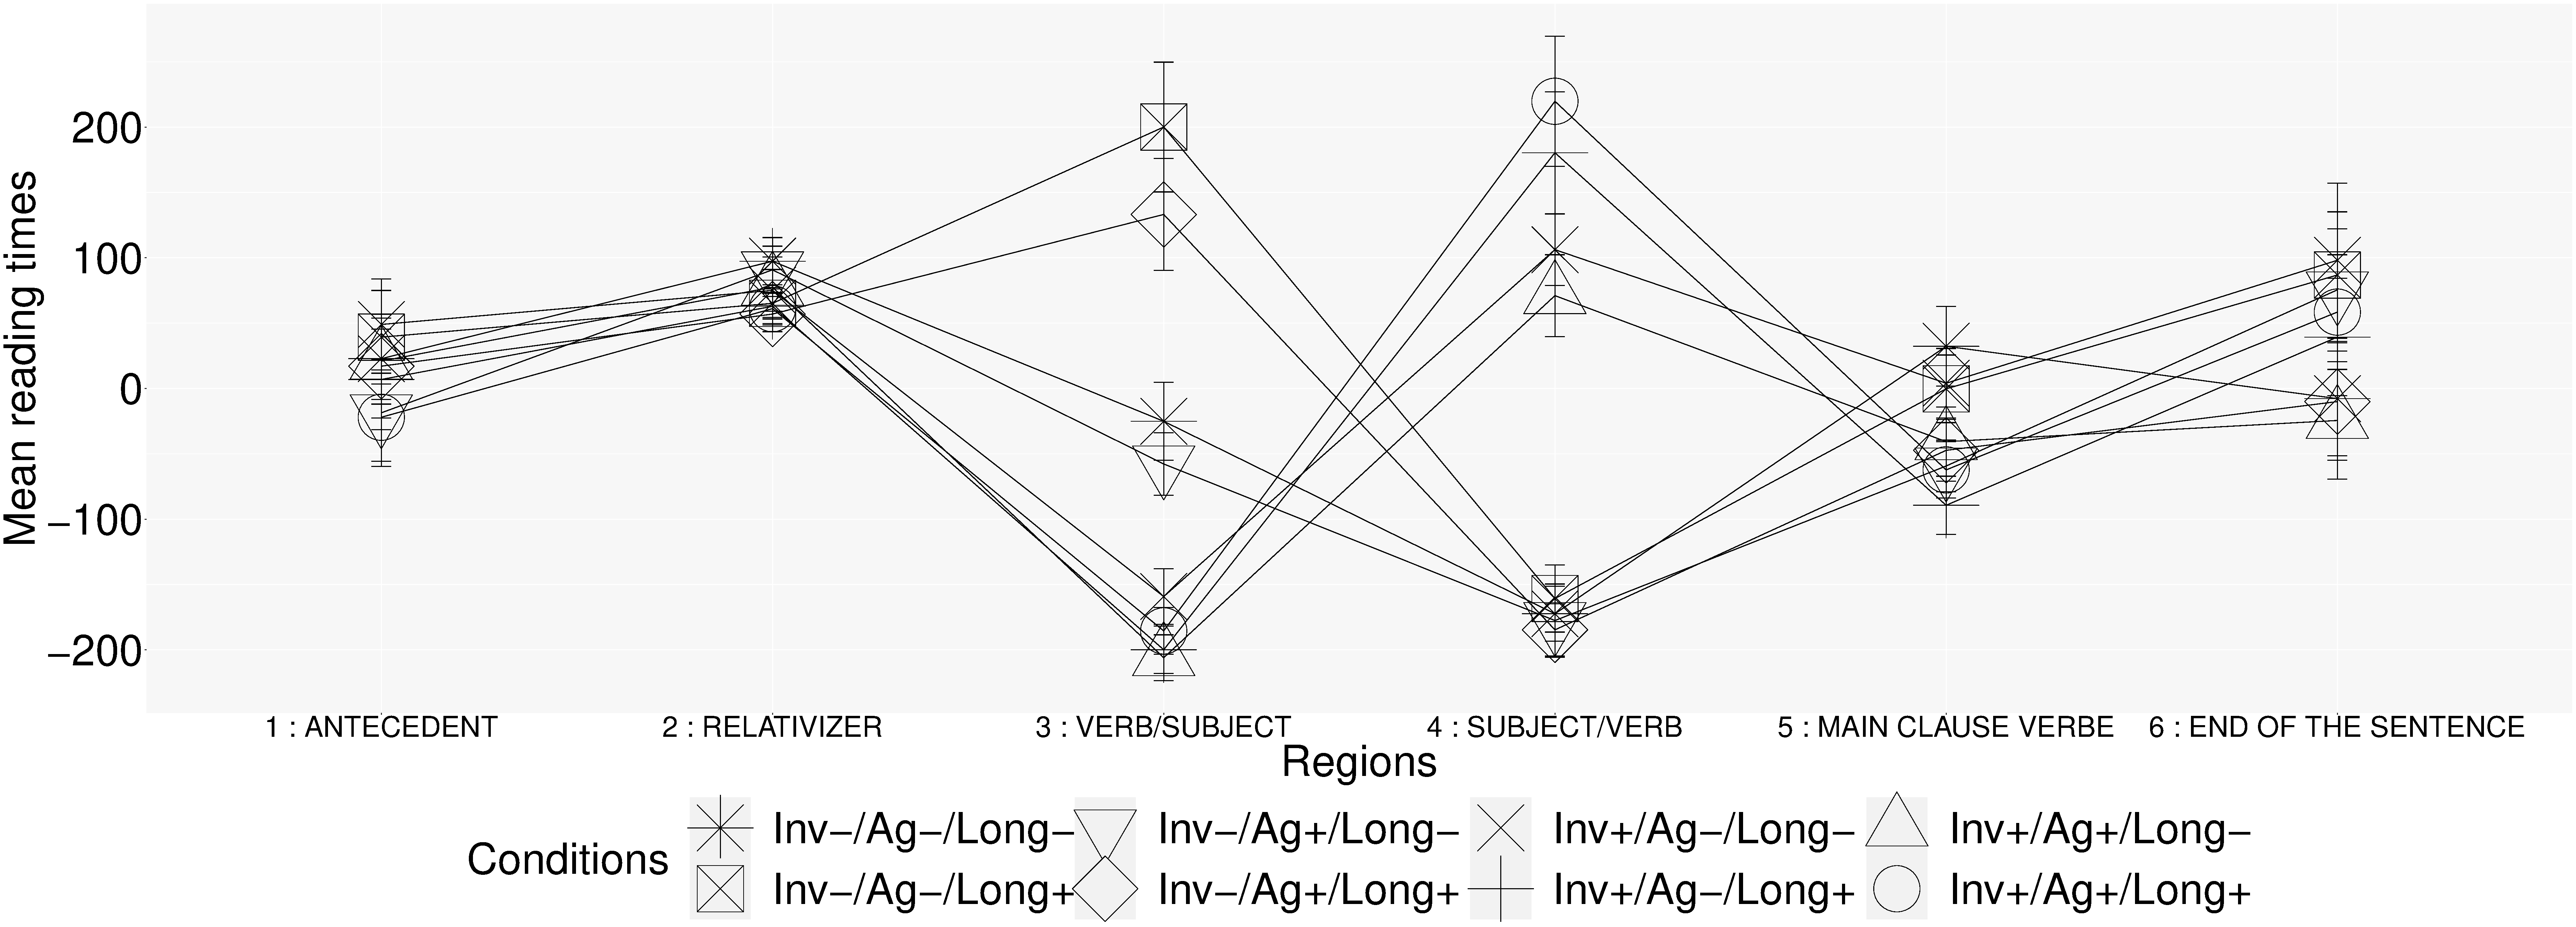
\includegraphics[width=\textwidth]{figures/PozHemAb4.pdf}
\caption{Residual reading times for the eight conditions in each region of the sentences}
\label{figureselfpacedallresults}
\end{figure}


In this paper, we focus on region 5 (main clause verb) since this region is identical across conditions. It appears after the relative clause and may show differences in processing. Figure \ref{figureselfpacedregion5} represents mean residual reading times for the main clause verb (region 5).

\begin{figure}
    \resizebox{\linewidth}{!}{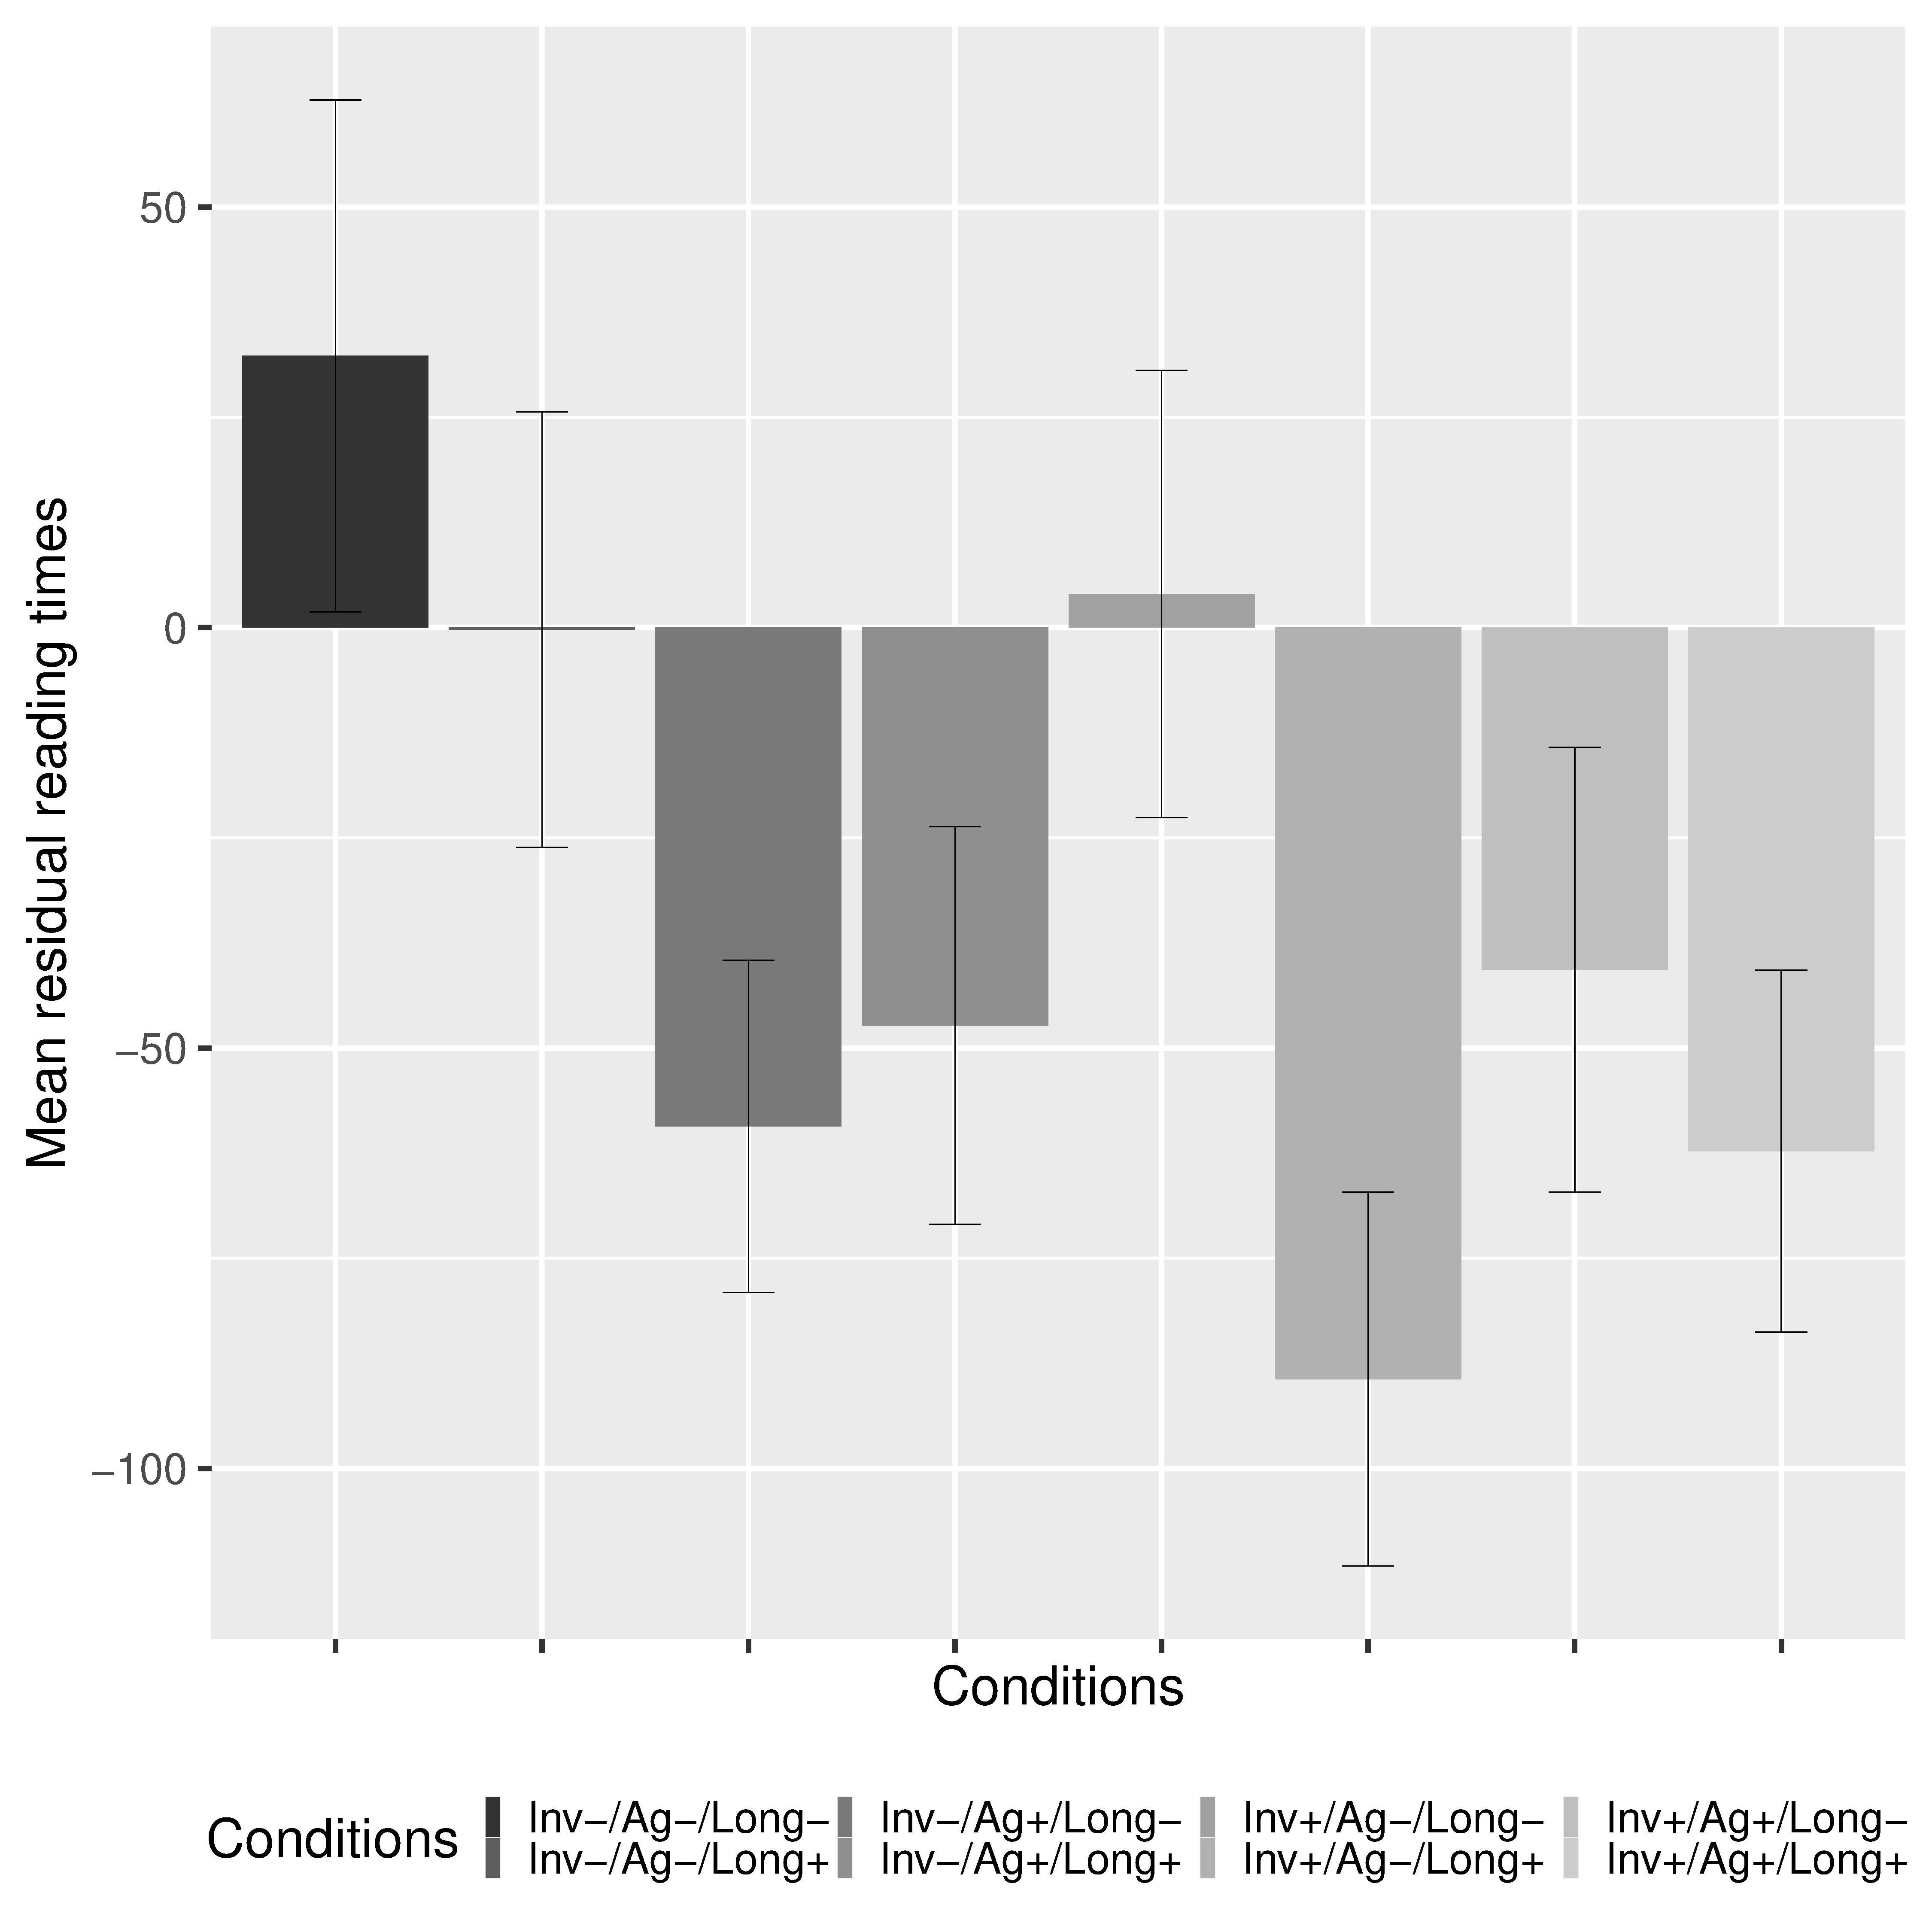
\includegraphics{figures/PozHemAb5.pdf}}
\caption{Mean residual reading times in the main verb region. Error bars represent standard errors.}
\label{figureselfpacedregion5}
\end{figure}

In region 5 (\figref{figureselfpacedregion5}), we found a general effect of verb semantics ($t=2.26,\allowbreak p<0.05$): reading non-agentive verbs took longer than reading agentive verbs. An interaction between subject length and verb semantics is also observed ($t=2.59,\allowbreak p<0.05$): reading times are longer with short subjects and non-agentive verbs compared to long subjects and agentive verbs. We also found a marginal effect of subject position ($t=-1.81, p=0.08$): relatives with a postverbal subject seem to be read faster than relatives with a preverbal subject. 


Interestingly, when subsetting relatives with postverbal subject, we found an effect of subject length ($t=-2.06, p<0.05$) as well as an interaction between verb agentivity and subject length ($t=-3.08, p<0.01$).\footnote{We had to remove the interaction of the fixed factors in the random variables to make the model converge: \texttt{m1=lmer(log(reaction) $\sim$ Sémantique $+$ Longueur $+$ length $+$ (Sémantique*Longueur $+$ 1||sujet) + (Sémantique $+$ Longueur $+$ 1 ||item), 
 data=inversion, control = lmerControl(optimizer = "optimx", calc.derivs = FALSE,optCtrl = list(method = "nlminb", starttests = FALSE, kkt = FALSE)))} }
This means that when the verb is not agentive, relatives are read faster with a long subject rather than with a short subject, whereas there is no difference in relatives with agentive verbs. Non-agentive verbs with long subjects correspond to the most felicitous context in the corpus study for relatives with postverbal subject. As for relatives with preverbal subject, an effect of verb semantics is found ($t=-2.70, p<0.05$): relatives with preverbal subject are read faster when the verb is agentive. 

 
 
 
\subsection{Interim discussion}
As in the acceptability judgements, object relatives with a postverbal subject are no more difficult to process than object relatives with a preverbal subject in our study -- contra \citet{Holmes1981}, \citet{pozniak2015processing}. The self-paced reading study also showed an effect of length and semantics in the main clause verb region (just after the relative): relatives with a short, preverbal subject and an agentive verb are read faster than when the verb is not agentive. Reading times in the same region showed that relatives with a long, postverbal subject and a non-agentive verb are easier to process than when the subject is short. Both of these combinations echo the specific conditions for pre- and postverbal subjects that we identified in the corpus analysis. Overall, the experiment suggests that subject length and verb semantics play a role in the position of the subject in object relative clauses. 

\section{Discussion and conclusions}

Predictions and data on the usage of object relative clauses with postverbal subject in French are inconsistent in the linguistic as well as in the psycholinguistic literature. There seems to be some general understanding that they are marked, more complex, less frequent and harder to understand than object relatives with preverbal subject. This general understanding, however, goes against predictions of some syntactic approaches \citep [e.g. relativized minimality,] []{rizzi1990} as well as some psycholinguistic processing theories \citep [e.g. DLT,] []{gibson2000}. Previous qualitative corpus studies \citep{catherine1997} as well as psycholinguistic experiments point to an even more complex picture where a variety of constraints has to be taken into account.

This inconsistency in the literature led us to the hypothesis that treating object relative clauses with pre- or postverbal subject as just two more or less complex or marked variants may be the wrong approach. What if these two variants are not basically different in acceptability or processing complexity but just favored by different sets of properties?  Increased processing complexity of ORs with postverbal subject would then be the consequence of using materials more adapted to ORs with preverbal subject. Testing this hypothesis requires an approach based on controlled empirical data. Therefore, we decided to run a written corpus study, followed by acceptability judgements and a self-paced reading experiment.

Contrary to previous corpus studies \citep{catherine1997}, who claimed a slight advantage for preverbal subject overall (all relatives confounded), we found that subject inversion can be as frequent as preverbal subjects in French object relatives under fully controlled conditions. Thus, frequency per se does not predict a preference for one or the other as was found in \citet{Frauenfelder1980} or \citet{pozniak2015processing}.

Corpus annotation on the French Treebank \citep{abeille2019corpus} also shows that object relatives with preverbal and postverbal subjects have different properties and are used in different contexts. Logistic regression models \citep{baayen2008mixed} show that semantic factors (agentivity and intentionality) as well as length play a significant role in subject inversion. 

In order to see whether these properties differentiate object relatives with preverbal and postverbal subject, we manipulated them in two experimental studies: an acceptability judgement study and a self-paced reading experiment. The acceptability judgement experiment shows that subject inversion is rated highly acceptable and might even be preferred in object relative clauses under the right circumstances, contrary to previous experimental studies \citep{Holmes1981, pozniak2015processing}. The self-paced reading experiment shows that verb agentivity and subject length both play a role in the use of object relatives with preverbal subject and with postverbal subject. A non-agentive verb and a long subject make OR$+$inv easier to process. However, we did not test other semantic factors such as object definiteness. More experiments examining semantic and discourse factors are needed to complete the picture. The results of our experiments were also not as clear cut as we might have wished. This may be due to the fact that they were run on an internet platform, where the experimental environment is much less controlled than in the lab.

Overall, our results cannot be explained by theories which would consider postverbal subjects generally more complex than preverbal subjects as proposed by some of the syntactic theories mentioned in the introduction. They cannot be explained either by processing theories such as DLT, which predicts a systematic advantage for subject inversion, or by syntactic theories like relativized minimality that may similarly predict an advantage for inversion.  Depending on semantic properties, object relatives with a postverbal subject are not always easier or harder to understand than object relatives with a preverbal subject as suggested in the psycholinguistic literature, which is mainly focused on reversible relative clauses with animate subjects and objects, mostly using agentive verbs \citep{Holmes1981, pozniak2015processing}.

To conclude, our three empirical studies emphasize the role of length and semantic/pragmatic factors \citep{mak2006animacy, traxler2002}. The role of subject length could be explained by dependency locality theory \citep{gibson2000} or by a more general tendency to put longer constituents at the end of the sentence \citep{Behaghel, wasow2002postverbal}.  The role of verb agentivity could be explained by semantic theories \citep{Fuchs2006, marandin2011}. 

Our studies also show that subject inversion is not marked and is no less frequent than preverbal subjects in French object relatives. Relatives with postverbal subject, which existed in Ancient French \citep{buridant1999ordre, fuchs2006franccais} coexist now with relatives with preverbal subject and can be felicitous depending on their semantic/pragmatic properties. Thus, we propose that subject inversion is not just a stylistic variant. Object relatives with preverbal or postverbal subject can be seen as two variants of a grammatical construction with different usage profiles and each can be more appropriate than the other in the right context.


\section*{Abbreviations}
\begin{tabular}{@{}ll@{}}
OR & Object relative\\
OR$+$inv & Object relative with subject inversion \\
OR$-$inv & Object relative without subject inversion\\
DLT & Dependency locality theory \\
\end{tabular}

\section*{Acknowledgements}
We thank Clément Plancq for extracting the relative clauses from the French Treebank as well as Jean-Marie Marandin for very helpful discussions. We also thank the Procope Paris--Frankurt project \textit{One2Many} for its help. This work was partially supported by a public grant overseen by the French National Research Agency (ANR) as part of the program “Investissements d’Avenir” (reference: ANR-10-LABX-0083). It contributes to the IdEx Université de Paris – ANR-18-IDEX-0001.

{\sloppy\printbibliography[heading=subbibliography,notkeyword=this]}

\end{document}
